
    




    
\documentclass[11pt]{article}

    
    \usepackage[breakable]{tcolorbox}
    \tcbset{nobeforeafter} % prevents tcolorboxes being placing in paragraphs
    \usepackage{float}
    \floatplacement{figure}{H} % forces figures to be placed at the correct location
    
    \usepackage[T1]{fontenc}
    % Nicer default font (+ math font) than Computer Modern for most use cases
    \usepackage{mathpazo}

    % Basic figure setup, for now with no caption control since it's done
    % automatically by Pandoc (which extracts ![](path) syntax from Markdown).
    \usepackage{graphicx}
    % We will generate all images so they have a width \maxwidth. This means
    % that they will get their normal width if they fit onto the page, but
    % are scaled down if they would overflow the margins.
    \makeatletter
    \def\maxwidth{\ifdim\Gin@nat@width>\linewidth\linewidth
    \else\Gin@nat@width\fi}
    \makeatother
    \let\Oldincludegraphics\includegraphics
    % Set max figure width to be 80% of text width, for now hardcoded.
    \renewcommand{\includegraphics}[1]{\Oldincludegraphics[width=.8\maxwidth]{#1}}
    % Ensure that by default, figures have no caption (until we provide a
    % proper Figure object with a Caption API and a way to capture that
    % in the conversion process - todo).
    \usepackage{caption}
    \DeclareCaptionLabelFormat{nolabel}{}
    \captionsetup{labelformat=nolabel}

    \usepackage{adjustbox} % Used to constrain images to a maximum size 
    \usepackage{xcolor} % Allow colors to be defined
    \usepackage{enumerate} % Needed for markdown enumerations to work
    \usepackage{geometry} % Used to adjust the document margins
    \usepackage{amsmath} % Equations
    \usepackage{amssymb} % Equations
    \usepackage{textcomp} % defines textquotesingle
    % Hack from http://tex.stackexchange.com/a/47451/13684:
    \AtBeginDocument{%
        \def\PYZsq{\textquotesingle}% Upright quotes in Pygmentized code
    }
    \usepackage{upquote} % Upright quotes for verbatim code
    \usepackage{eurosym} % defines \euro
    \usepackage[mathletters]{ucs} % Extended unicode (utf-8) support
    \usepackage[utf8x]{inputenc} % Allow utf-8 characters in the tex document
    \usepackage{fancyvrb} % verbatim replacement that allows latex
    \usepackage{grffile} % extends the file name processing of package graphics 
                         % to support a larger range 
    % The hyperref package gives us a pdf with properly built
    % internal navigation ('pdf bookmarks' for the table of contents,
    % internal cross-reference links, web links for URLs, etc.)
    \usepackage{hyperref}
    \usepackage{longtable} % longtable support required by pandoc >1.10
    \usepackage{booktabs}  % table support for pandoc > 1.12.2
    \usepackage[inline]{enumitem} % IRkernel/repr support (it uses the enumerate* environment)
    \usepackage[normalem]{ulem} % ulem is needed to support strikethroughs (\sout)
                                % normalem makes italics be italics, not underlines
    \usepackage{mathrsfs}
    

    
    % Colors for the hyperref package
    \definecolor{urlcolor}{rgb}{0,.145,.698}
    \definecolor{linkcolor}{rgb}{.71,0.21,0.01}
    \definecolor{citecolor}{rgb}{.12,.54,.11}

    % ANSI colors
    \definecolor{ansi-black}{HTML}{3E424D}
    \definecolor{ansi-black-intense}{HTML}{282C36}
    \definecolor{ansi-red}{HTML}{E75C58}
    \definecolor{ansi-red-intense}{HTML}{B22B31}
    \definecolor{ansi-green}{HTML}{00A250}
    \definecolor{ansi-green-intense}{HTML}{007427}
    \definecolor{ansi-yellow}{HTML}{DDB62B}
    \definecolor{ansi-yellow-intense}{HTML}{B27D12}
    \definecolor{ansi-blue}{HTML}{208FFB}
    \definecolor{ansi-blue-intense}{HTML}{0065CA}
    \definecolor{ansi-magenta}{HTML}{D160C4}
    \definecolor{ansi-magenta-intense}{HTML}{A03196}
    \definecolor{ansi-cyan}{HTML}{60C6C8}
    \definecolor{ansi-cyan-intense}{HTML}{258F8F}
    \definecolor{ansi-white}{HTML}{C5C1B4}
    \definecolor{ansi-white-intense}{HTML}{A1A6B2}
    \definecolor{ansi-default-inverse-fg}{HTML}{FFFFFF}
    \definecolor{ansi-default-inverse-bg}{HTML}{000000}

    % commands and environments needed by pandoc snippets
    % extracted from the output of `pandoc -s`
    \providecommand{\tightlist}{%
      \setlength{\itemsep}{0pt}\setlength{\parskip}{0pt}}
    \DefineVerbatimEnvironment{Highlighting}{Verbatim}{commandchars=\\\{\}}
    % Add ',fontsize=\small' for more characters per line
    \newenvironment{Shaded}{}{}
    \newcommand{\KeywordTok}[1]{\textcolor[rgb]{0.00,0.44,0.13}{\textbf{{#1}}}}
    \newcommand{\DataTypeTok}[1]{\textcolor[rgb]{0.56,0.13,0.00}{{#1}}}
    \newcommand{\DecValTok}[1]{\textcolor[rgb]{0.25,0.63,0.44}{{#1}}}
    \newcommand{\BaseNTok}[1]{\textcolor[rgb]{0.25,0.63,0.44}{{#1}}}
    \newcommand{\FloatTok}[1]{\textcolor[rgb]{0.25,0.63,0.44}{{#1}}}
    \newcommand{\CharTok}[1]{\textcolor[rgb]{0.25,0.44,0.63}{{#1}}}
    \newcommand{\StringTok}[1]{\textcolor[rgb]{0.25,0.44,0.63}{{#1}}}
    \newcommand{\CommentTok}[1]{\textcolor[rgb]{0.38,0.63,0.69}{\textit{{#1}}}}
    \newcommand{\OtherTok}[1]{\textcolor[rgb]{0.00,0.44,0.13}{{#1}}}
    \newcommand{\AlertTok}[1]{\textcolor[rgb]{1.00,0.00,0.00}{\textbf{{#1}}}}
    \newcommand{\FunctionTok}[1]{\textcolor[rgb]{0.02,0.16,0.49}{{#1}}}
    \newcommand{\RegionMarkerTok}[1]{{#1}}
    \newcommand{\ErrorTok}[1]{\textcolor[rgb]{1.00,0.00,0.00}{\textbf{{#1}}}}
    \newcommand{\NormalTok}[1]{{#1}}
    
    % Additional commands for more recent versions of Pandoc
    \newcommand{\ConstantTok}[1]{\textcolor[rgb]{0.53,0.00,0.00}{{#1}}}
    \newcommand{\SpecialCharTok}[1]{\textcolor[rgb]{0.25,0.44,0.63}{{#1}}}
    \newcommand{\VerbatimStringTok}[1]{\textcolor[rgb]{0.25,0.44,0.63}{{#1}}}
    \newcommand{\SpecialStringTok}[1]{\textcolor[rgb]{0.73,0.40,0.53}{{#1}}}
    \newcommand{\ImportTok}[1]{{#1}}
    \newcommand{\DocumentationTok}[1]{\textcolor[rgb]{0.73,0.13,0.13}{\textit{{#1}}}}
    \newcommand{\AnnotationTok}[1]{\textcolor[rgb]{0.38,0.63,0.69}{\textbf{\textit{{#1}}}}}
    \newcommand{\CommentVarTok}[1]{\textcolor[rgb]{0.38,0.63,0.69}{\textbf{\textit{{#1}}}}}
    \newcommand{\VariableTok}[1]{\textcolor[rgb]{0.10,0.09,0.49}{{#1}}}
    \newcommand{\ControlFlowTok}[1]{\textcolor[rgb]{0.00,0.44,0.13}{\textbf{{#1}}}}
    \newcommand{\OperatorTok}[1]{\textcolor[rgb]{0.40,0.40,0.40}{{#1}}}
    \newcommand{\BuiltInTok}[1]{{#1}}
    \newcommand{\ExtensionTok}[1]{{#1}}
    \newcommand{\PreprocessorTok}[1]{\textcolor[rgb]{0.74,0.48,0.00}{{#1}}}
    \newcommand{\AttributeTok}[1]{\textcolor[rgb]{0.49,0.56,0.16}{{#1}}}
    \newcommand{\InformationTok}[1]{\textcolor[rgb]{0.38,0.63,0.69}{\textbf{\textit{{#1}}}}}
    \newcommand{\WarningTok}[1]{\textcolor[rgb]{0.38,0.63,0.69}{\textbf{\textit{{#1}}}}}
    
    
    % Define a nice break command that doesn't care if a line doesn't already
    % exist.
    \def\br{\hspace*{\fill} \\* }
    % Math Jax compatibility definitions
    \def\gt{>}
    \def\lt{<}
    \let\Oldtex\TeX
    \let\Oldlatex\LaTeX
    \renewcommand{\TeX}{\textrm{\Oldtex}}
    \renewcommand{\LaTeX}{\textrm{\Oldlatex}}
    % Document parameters
    % Document title
    \title{	
	\normalfont\normalsize
	\textsc{ 5CL}\ % Your university, school and/or department name(s)
	\vspace{25pt} % Whitespace
	\rule{\linewidth}{0.5pt}\ % Thin top horizontal rule
	\vspace{20pt} % Whitespace
	{\huge Lab 5: The Photoelectric Effect}\ % The assignment title
	\vspace{12pt} % Whitespace
	\rule{\linewidth}{2pt}\ % Thick bottom horizontal rule
	\vspace{12pt} % Whitespace
}

\author{\LARGE Daniel Geisz \& Heidi Hu} % Your name

\date{\normalsize\today}
    
    
    
    
    
% Pygments definitions
\makeatletter
\def\PY@reset{\let\PY@it=\relax \let\PY@bf=\relax%
    \let\PY@ul=\relax \let\PY@tc=\relax%
    \let\PY@bc=\relax \let\PY@ff=\relax}
\def\PY@tok#1{\csname PY@tok@#1\endcsname}
\def\PY@toks#1+{\ifx\relax#1\empty\else%
    \PY@tok{#1}\expandafter\PY@toks\fi}
\def\PY@do#1{\PY@bc{\PY@tc{\PY@ul{%
    \PY@it{\PY@bf{\PY@ff{#1}}}}}}}
\def\PY#1#2{\PY@reset\PY@toks#1+\relax+\PY@do{#2}}

\expandafter\def\csname PY@tok@w\endcsname{\def\PY@tc##1{\textcolor[rgb]{0.73,0.73,0.73}{##1}}}
\expandafter\def\csname PY@tok@c\endcsname{\let\PY@it=\textit\def\PY@tc##1{\textcolor[rgb]{0.25,0.50,0.50}{##1}}}
\expandafter\def\csname PY@tok@cp\endcsname{\def\PY@tc##1{\textcolor[rgb]{0.74,0.48,0.00}{##1}}}
\expandafter\def\csname PY@tok@k\endcsname{\let\PY@bf=\textbf\def\PY@tc##1{\textcolor[rgb]{0.00,0.50,0.00}{##1}}}
\expandafter\def\csname PY@tok@kp\endcsname{\def\PY@tc##1{\textcolor[rgb]{0.00,0.50,0.00}{##1}}}
\expandafter\def\csname PY@tok@kt\endcsname{\def\PY@tc##1{\textcolor[rgb]{0.69,0.00,0.25}{##1}}}
\expandafter\def\csname PY@tok@o\endcsname{\def\PY@tc##1{\textcolor[rgb]{0.40,0.40,0.40}{##1}}}
\expandafter\def\csname PY@tok@ow\endcsname{\let\PY@bf=\textbf\def\PY@tc##1{\textcolor[rgb]{0.67,0.13,1.00}{##1}}}
\expandafter\def\csname PY@tok@nb\endcsname{\def\PY@tc##1{\textcolor[rgb]{0.00,0.50,0.00}{##1}}}
\expandafter\def\csname PY@tok@nf\endcsname{\def\PY@tc##1{\textcolor[rgb]{0.00,0.00,1.00}{##1}}}
\expandafter\def\csname PY@tok@nc\endcsname{\let\PY@bf=\textbf\def\PY@tc##1{\textcolor[rgb]{0.00,0.00,1.00}{##1}}}
\expandafter\def\csname PY@tok@nn\endcsname{\let\PY@bf=\textbf\def\PY@tc##1{\textcolor[rgb]{0.00,0.00,1.00}{##1}}}
\expandafter\def\csname PY@tok@ne\endcsname{\let\PY@bf=\textbf\def\PY@tc##1{\textcolor[rgb]{0.82,0.25,0.23}{##1}}}
\expandafter\def\csname PY@tok@nv\endcsname{\def\PY@tc##1{\textcolor[rgb]{0.10,0.09,0.49}{##1}}}
\expandafter\def\csname PY@tok@no\endcsname{\def\PY@tc##1{\textcolor[rgb]{0.53,0.00,0.00}{##1}}}
\expandafter\def\csname PY@tok@nl\endcsname{\def\PY@tc##1{\textcolor[rgb]{0.63,0.63,0.00}{##1}}}
\expandafter\def\csname PY@tok@ni\endcsname{\let\PY@bf=\textbf\def\PY@tc##1{\textcolor[rgb]{0.60,0.60,0.60}{##1}}}
\expandafter\def\csname PY@tok@na\endcsname{\def\PY@tc##1{\textcolor[rgb]{0.49,0.56,0.16}{##1}}}
\expandafter\def\csname PY@tok@nt\endcsname{\let\PY@bf=\textbf\def\PY@tc##1{\textcolor[rgb]{0.00,0.50,0.00}{##1}}}
\expandafter\def\csname PY@tok@nd\endcsname{\def\PY@tc##1{\textcolor[rgb]{0.67,0.13,1.00}{##1}}}
\expandafter\def\csname PY@tok@s\endcsname{\def\PY@tc##1{\textcolor[rgb]{0.73,0.13,0.13}{##1}}}
\expandafter\def\csname PY@tok@sd\endcsname{\let\PY@it=\textit\def\PY@tc##1{\textcolor[rgb]{0.73,0.13,0.13}{##1}}}
\expandafter\def\csname PY@tok@si\endcsname{\let\PY@bf=\textbf\def\PY@tc##1{\textcolor[rgb]{0.73,0.40,0.53}{##1}}}
\expandafter\def\csname PY@tok@se\endcsname{\let\PY@bf=\textbf\def\PY@tc##1{\textcolor[rgb]{0.73,0.40,0.13}{##1}}}
\expandafter\def\csname PY@tok@sr\endcsname{\def\PY@tc##1{\textcolor[rgb]{0.73,0.40,0.53}{##1}}}
\expandafter\def\csname PY@tok@ss\endcsname{\def\PY@tc##1{\textcolor[rgb]{0.10,0.09,0.49}{##1}}}
\expandafter\def\csname PY@tok@sx\endcsname{\def\PY@tc##1{\textcolor[rgb]{0.00,0.50,0.00}{##1}}}
\expandafter\def\csname PY@tok@m\endcsname{\def\PY@tc##1{\textcolor[rgb]{0.40,0.40,0.40}{##1}}}
\expandafter\def\csname PY@tok@gh\endcsname{\let\PY@bf=\textbf\def\PY@tc##1{\textcolor[rgb]{0.00,0.00,0.50}{##1}}}
\expandafter\def\csname PY@tok@gu\endcsname{\let\PY@bf=\textbf\def\PY@tc##1{\textcolor[rgb]{0.50,0.00,0.50}{##1}}}
\expandafter\def\csname PY@tok@gd\endcsname{\def\PY@tc##1{\textcolor[rgb]{0.63,0.00,0.00}{##1}}}
\expandafter\def\csname PY@tok@gi\endcsname{\def\PY@tc##1{\textcolor[rgb]{0.00,0.63,0.00}{##1}}}
\expandafter\def\csname PY@tok@gr\endcsname{\def\PY@tc##1{\textcolor[rgb]{1.00,0.00,0.00}{##1}}}
\expandafter\def\csname PY@tok@ge\endcsname{\let\PY@it=\textit}
\expandafter\def\csname PY@tok@gs\endcsname{\let\PY@bf=\textbf}
\expandafter\def\csname PY@tok@gp\endcsname{\let\PY@bf=\textbf\def\PY@tc##1{\textcolor[rgb]{0.00,0.00,0.50}{##1}}}
\expandafter\def\csname PY@tok@go\endcsname{\def\PY@tc##1{\textcolor[rgb]{0.53,0.53,0.53}{##1}}}
\expandafter\def\csname PY@tok@gt\endcsname{\def\PY@tc##1{\textcolor[rgb]{0.00,0.27,0.87}{##1}}}
\expandafter\def\csname PY@tok@err\endcsname{\def\PY@bc##1{\setlength{\fboxsep}{0pt}\fcolorbox[rgb]{1.00,0.00,0.00}{1,1,1}{\strut ##1}}}
\expandafter\def\csname PY@tok@kc\endcsname{\let\PY@bf=\textbf\def\PY@tc##1{\textcolor[rgb]{0.00,0.50,0.00}{##1}}}
\expandafter\def\csname PY@tok@kd\endcsname{\let\PY@bf=\textbf\def\PY@tc##1{\textcolor[rgb]{0.00,0.50,0.00}{##1}}}
\expandafter\def\csname PY@tok@kn\endcsname{\let\PY@bf=\textbf\def\PY@tc##1{\textcolor[rgb]{0.00,0.50,0.00}{##1}}}
\expandafter\def\csname PY@tok@kr\endcsname{\let\PY@bf=\textbf\def\PY@tc##1{\textcolor[rgb]{0.00,0.50,0.00}{##1}}}
\expandafter\def\csname PY@tok@bp\endcsname{\def\PY@tc##1{\textcolor[rgb]{0.00,0.50,0.00}{##1}}}
\expandafter\def\csname PY@tok@fm\endcsname{\def\PY@tc##1{\textcolor[rgb]{0.00,0.00,1.00}{##1}}}
\expandafter\def\csname PY@tok@vc\endcsname{\def\PY@tc##1{\textcolor[rgb]{0.10,0.09,0.49}{##1}}}
\expandafter\def\csname PY@tok@vg\endcsname{\def\PY@tc##1{\textcolor[rgb]{0.10,0.09,0.49}{##1}}}
\expandafter\def\csname PY@tok@vi\endcsname{\def\PY@tc##1{\textcolor[rgb]{0.10,0.09,0.49}{##1}}}
\expandafter\def\csname PY@tok@vm\endcsname{\def\PY@tc##1{\textcolor[rgb]{0.10,0.09,0.49}{##1}}}
\expandafter\def\csname PY@tok@sa\endcsname{\def\PY@tc##1{\textcolor[rgb]{0.73,0.13,0.13}{##1}}}
\expandafter\def\csname PY@tok@sb\endcsname{\def\PY@tc##1{\textcolor[rgb]{0.73,0.13,0.13}{##1}}}
\expandafter\def\csname PY@tok@sc\endcsname{\def\PY@tc##1{\textcolor[rgb]{0.73,0.13,0.13}{##1}}}
\expandafter\def\csname PY@tok@dl\endcsname{\def\PY@tc##1{\textcolor[rgb]{0.73,0.13,0.13}{##1}}}
\expandafter\def\csname PY@tok@s2\endcsname{\def\PY@tc##1{\textcolor[rgb]{0.73,0.13,0.13}{##1}}}
\expandafter\def\csname PY@tok@sh\endcsname{\def\PY@tc##1{\textcolor[rgb]{0.73,0.13,0.13}{##1}}}
\expandafter\def\csname PY@tok@s1\endcsname{\def\PY@tc##1{\textcolor[rgb]{0.73,0.13,0.13}{##1}}}
\expandafter\def\csname PY@tok@mb\endcsname{\def\PY@tc##1{\textcolor[rgb]{0.40,0.40,0.40}{##1}}}
\expandafter\def\csname PY@tok@mf\endcsname{\def\PY@tc##1{\textcolor[rgb]{0.40,0.40,0.40}{##1}}}
\expandafter\def\csname PY@tok@mh\endcsname{\def\PY@tc##1{\textcolor[rgb]{0.40,0.40,0.40}{##1}}}
\expandafter\def\csname PY@tok@mi\endcsname{\def\PY@tc##1{\textcolor[rgb]{0.40,0.40,0.40}{##1}}}
\expandafter\def\csname PY@tok@il\endcsname{\def\PY@tc##1{\textcolor[rgb]{0.40,0.40,0.40}{##1}}}
\expandafter\def\csname PY@tok@mo\endcsname{\def\PY@tc##1{\textcolor[rgb]{0.40,0.40,0.40}{##1}}}
\expandafter\def\csname PY@tok@ch\endcsname{\let\PY@it=\textit\def\PY@tc##1{\textcolor[rgb]{0.25,0.50,0.50}{##1}}}
\expandafter\def\csname PY@tok@cm\endcsname{\let\PY@it=\textit\def\PY@tc##1{\textcolor[rgb]{0.25,0.50,0.50}{##1}}}
\expandafter\def\csname PY@tok@cpf\endcsname{\let\PY@it=\textit\def\PY@tc##1{\textcolor[rgb]{0.25,0.50,0.50}{##1}}}
\expandafter\def\csname PY@tok@c1\endcsname{\let\PY@it=\textit\def\PY@tc##1{\textcolor[rgb]{0.25,0.50,0.50}{##1}}}
\expandafter\def\csname PY@tok@cs\endcsname{\let\PY@it=\textit\def\PY@tc##1{\textcolor[rgb]{0.25,0.50,0.50}{##1}}}

\def\PYZbs{\char`\\}
\def\PYZus{\char`\_}
\def\PYZob{\char`\{}
\def\PYZcb{\char`\}}
\def\PYZca{\char`\^}
\def\PYZam{\char`\&}
\def\PYZlt{\char`\<}
\def\PYZgt{\char`\>}
\def\PYZsh{\char`\#}
\def\PYZpc{\char`\%}
\def\PYZdl{\char`\$}
\def\PYZhy{\char`\-}
\def\PYZsq{\char`\'}
\def\PYZdq{\char`\"}
\def\PYZti{\char`\~}
% for compatibility with earlier versions
\def\PYZat{@}
\def\PYZlb{[}
\def\PYZrb{]}
\makeatother


    % For linebreaks inside Verbatim environment from package fancyvrb. 
    \makeatletter
        \newbox\Wrappedcontinuationbox 
        \newbox\Wrappedvisiblespacebox 
        \newcommand*\Wrappedvisiblespace {\textcolor{red}{\textvisiblespace}} 
        \newcommand*\Wrappedcontinuationsymbol {\textcolor{red}{\llap{\tiny$\m@th\hookrightarrow$}}} 
        \newcommand*\Wrappedcontinuationindent {3ex } 
        \newcommand*\Wrappedafterbreak {\kern\Wrappedcontinuationindent\copy\Wrappedcontinuationbox} 
        % Take advantage of the already applied Pygments mark-up to insert 
        % potential linebreaks for TeX processing. 
        %        {, <, #, %, $, ' and ": go to next line. 
        %        _, }, ^, &, >, - and ~: stay at end of broken line. 
        % Use of \textquotesingle for straight quote. 
        \newcommand*\Wrappedbreaksatspecials {% 
            \def\PYGZus{\discretionary{\char`\_}{\Wrappedafterbreak}{\char`\_}}% 
            \def\PYGZob{\discretionary{}{\Wrappedafterbreak\char`\{}{\char`\{}}% 
            \def\PYGZcb{\discretionary{\char`\}}{\Wrappedafterbreak}{\char`\}}}% 
            \def\PYGZca{\discretionary{\char`\^}{\Wrappedafterbreak}{\char`\^}}% 
            \def\PYGZam{\discretionary{\char`\&}{\Wrappedafterbreak}{\char`\&}}% 
            \def\PYGZlt{\discretionary{}{\Wrappedafterbreak\char`\<}{\char`\<}}% 
            \def\PYGZgt{\discretionary{\char`\>}{\Wrappedafterbreak}{\char`\>}}% 
            \def\PYGZsh{\discretionary{}{\Wrappedafterbreak\char`\#}{\char`\#}}% 
            \def\PYGZpc{\discretionary{}{\Wrappedafterbreak\char`\%}{\char`\%}}% 
            \def\PYGZdl{\discretionary{}{\Wrappedafterbreak\char`\$}{\char`\$}}% 
            \def\PYGZhy{\discretionary{\char`\-}{\Wrappedafterbreak}{\char`\-}}% 
            \def\PYGZsq{\discretionary{}{\Wrappedafterbreak\textquotesingle}{\textquotesingle}}% 
            \def\PYGZdq{\discretionary{}{\Wrappedafterbreak\char`\"}{\char`\"}}% 
            \def\PYGZti{\discretionary{\char`\~}{\Wrappedafterbreak}{\char`\~}}% 
        } 
        % Some characters . , ; ? ! / are not pygmentized. 
        % This macro makes them "active" and they will insert potential linebreaks 
        \newcommand*\Wrappedbreaksatpunct {% 
            \lccode`\~`\.\lowercase{\def~}{\discretionary{\hbox{\char`\.}}{\Wrappedafterbreak}{\hbox{\char`\.}}}% 
            \lccode`\~`\,\lowercase{\def~}{\discretionary{\hbox{\char`\,}}{\Wrappedafterbreak}{\hbox{\char`\,}}}% 
            \lccode`\~`\;\lowercase{\def~}{\discretionary{\hbox{\char`\;}}{\Wrappedafterbreak}{\hbox{\char`\;}}}% 
            \lccode`\~`\:\lowercase{\def~}{\discretionary{\hbox{\char`\:}}{\Wrappedafterbreak}{\hbox{\char`\:}}}% 
            \lccode`\~`\?\lowercase{\def~}{\discretionary{\hbox{\char`\?}}{\Wrappedafterbreak}{\hbox{\char`\?}}}% 
            \lccode`\~`\!\lowercase{\def~}{\discretionary{\hbox{\char`\!}}{\Wrappedafterbreak}{\hbox{\char`\!}}}% 
            \lccode`\~`\/\lowercase{\def~}{\discretionary{\hbox{\char`\/}}{\Wrappedafterbreak}{\hbox{\char`\/}}}% 
            \catcode`\.\active
            \catcode`\,\active 
            \catcode`\;\active
            \catcode`\:\active
            \catcode`\?\active
            \catcode`\!\active
            \catcode`\/\active 
            \lccode`\~`\~ 	
        }
    \makeatother

    \let\OriginalVerbatim=\Verbatim
    \makeatletter
    \renewcommand{\Verbatim}[1][1]{%
        %\parskip\z@skip
        \sbox\Wrappedcontinuationbox {\Wrappedcontinuationsymbol}%
        \sbox\Wrappedvisiblespacebox {\FV@SetupFont\Wrappedvisiblespace}%
        \def\FancyVerbFormatLine ##1{\hsize\linewidth
            \vtop{\raggedright\hyphenpenalty\z@\exhyphenpenalty\z@
                \doublehyphendemerits\z@\finalhyphendemerits\z@
                \strut ##1\strut}%
        }%
        % If the linebreak is at a space, the latter will be displayed as visible
        % space at end of first line, and a continuation symbol starts next line.
        % Stretch/shrink are however usually zero for typewriter font.
        \def\FV@Space {%
            \nobreak\hskip\z@ plus\fontdimen3\font minus\fontdimen4\font
            \discretionary{\copy\Wrappedvisiblespacebox}{\Wrappedafterbreak}
            {\kern\fontdimen2\font}%
        }%
        
        % Allow breaks at special characters using \PYG... macros.
        \Wrappedbreaksatspecials
        % Breaks at punctuation characters . , ; ? ! and / need catcode=\active 	
        \OriginalVerbatim[#1,codes*=\Wrappedbreaksatpunct]%
    }
    \makeatother

    % Exact colors from NB
    \definecolor{incolor}{HTML}{303F9F}
    \definecolor{outcolor}{HTML}{D84315}
    \definecolor{cellborder}{HTML}{CFCFCF}
    \definecolor{cellbackground}{HTML}{F7F7F7}
    
    % prompt
    \newcommand{\prompt}[4]{
        \llap{{\color{#2}[#3]: #4}}\vspace{-1.25em}
    }
    

    
    % Prevent overflowing lines due to hard-to-break entities
    \sloppy 
    % Setup hyperref package
    \hypersetup{
      breaklinks=true,  % so long urls are correctly broken across lines
      colorlinks=true,
      urlcolor=urlcolor,
      linkcolor=linkcolor,
      citecolor=citecolor,
      }
    % Slightly bigger margins than the latex defaults
    
    \geometry{verbose,tmargin=1in,bmargin=1in,lmargin=1in,rmargin=1in}
    
    

    \begin{document}
    
    
    \maketitle
    
    

    
    \hypertarget{experiment-3---measuring-h-and-phi-with-leds}{%
\section{\texorpdfstring{Experiment 3 - Measuring \(h\) and \(\phi\)
with
LEDs}{Experiment 3 - Measuring h and \textbackslash phi with LEDs}}\label{experiment-3---measuring-h-and-phi-with-leds}}

\hypertarget{objective}{%
\subsection{Objective:}\label{objective}}

\begin{itemize}
\tightlist
\item
  We will use the photoelectric effect to determine Plank's constant
  \(h\), and the work function \(\phi\) and cutoff frequency \(f_o\) of
  the semiconductor in the phototube.
\end{itemize}

\hypertarget{method}{%
\subsection{Method:}\label{method}}

The main equation we use in this experiment is the photoelectric effect
equation:

\[K_{max} = hf - \phi\]

We also have:

\[K_{max} = eV_{stop}\]

So therefore,

\[eV_{stop} = hf - \phi\]

We also define the cutoff frequency \(f_o\) as the frequency at which
the photocurrent goes to zero. \(f_o\) is given theoretically as:

\[f_o = \frac{\phi}{h}\]

In order to determine \(h\), \(\phi\), and \(f_o\), we will find
\(V_{stop}\) for each of the LEDs and perform a linear fit on our data.

To start this experiment, we set up materials according to the section
``The Photoelectric Effect Setup'' in the lab manual. We then calibrated
the apparatus using the procedure specified in the lab manual. For each
of the LEDs, we took a series of data points from which we were able to
determine \(V_{stop}\). At that point, finding \(h\), \(\phi\), and
\(f_o\) is simply a matter of data analysis.

\hypertarget{data-analysis}{%
\subsection{Data Analysis:}\label{data-analysis}}

\begin{enumerate}
\def\labelenumi{\alph{enumi})}
\tightlist
\item
  Wavelengths: What wavelengths and uncertainties should we use for our
  LED data? Explain or justify
\end{enumerate}

In the previous experiment, we determined that the red LED had
wavelengths between 548 and 632 nm. That spread of wavelengths
corresponds to an uncertainty of \(\frac{(632 - 548) }{2} = 42\).
However, we noticed that these wavelengths actually correspond Orange,
Yellow, and Green light, so while we accurately measured the spread in
wavelengths, we believe that we did not properly measure the actual
wavelength. Because the Blue and Green LEDs had a similar spread in
wavelengths, we will use the listed value of wavelength in the lab
manual for each LED, and we will use an uncertainty of 42 nm to take
into account the spread over wavelengths for LEDs. Therefore:

$$
\text{Blue Wavelength: $462 \pm 42$ nm} $$
$$\text{Green Wavelength: $533\pm 42$ nm} $$
$$\text{Red Wavelength: $618 \pm 42$ nm}$$

\begin{enumerate}
\def\labelenumi{\alph{enumi})}
\setcounter{enumi}{1}
\tightlist
\item
  Stopping Voltage/Max KE: For each of the data sets, determine the
  stopping voltage with uncertainty. Describe how you are using your
  data to do so, including any necessary analyses.
\end{enumerate}

The following Data Tables and Graphs represent the Data we took for this
experiment. In each of the Data Tables, ``V'' represents the voltage
running through the photoelectric effect circuit in millivolts,
``Photocurrent'' of course refers to the photocurrent, as measured in
milliamps. ``delta\_pc'' refers to the uncertainty in the measurement of
the photocurrent.

Blue:

    \begin{tcolorbox}[breakable, size=fbox, boxrule=1pt, pad at break*=1mm,colback=cellbackground, colframe=cellborder]
\prompt{In}{incolor}{20}{\hspace{4pt}}
\begin{Verbatim}[commandchars=\\\{\}]
\PY{n}{blue}
\end{Verbatim}
\end{tcolorbox}

            \begin{tcolorbox}[breakable, boxrule=.5pt, size=fbox, pad at break*=1mm, opacityfill=0]
\prompt{Out}{outcolor}{20}{\hspace{3.5pt}}
\begin{Verbatim}[commandchars=\\\{\}]
     V  Photocurrent  delta\_pc
0 -931             0         1
1 -800           114         2
2 -700           321         2
3 -600           680         2
4 -500          1194         2
5 -300          2661         2
6 -100          4563         2
7    0          5598         2
8  200          7684         3
9  400          9779         2
\end{Verbatim}
\end{tcolorbox}
        
    \begin{tcolorbox}[breakable, size=fbox, boxrule=1pt, pad at break*=1mm,colback=cellbackground, colframe=cellborder]
\prompt{In}{incolor}{7}{\hspace{4pt}}
\begin{Verbatim}[commandchars=\\\{\}]
\PY{n}{plt}\PY{o}{.}\PY{n}{plot}\PY{p}{(}\PY{n}{blue}\PY{o}{.}\PY{n}{V}\PY{p}{,} \PY{n}{blue}\PY{o}{.}\PY{n}{Photocurrent}\PY{p}{)}
\PY{n}{plt}\PY{o}{.}\PY{n}{xlabel}\PY{p}{(}\PY{l+s+s2}{\PYZdq{}}\PY{l+s+s2}{Voltage (mv)}\PY{l+s+s2}{\PYZdq{}}\PY{p}{)}
\PY{n}{plt}\PY{o}{.}\PY{n}{ylabel}\PY{p}{(}\PY{l+s+s2}{\PYZdq{}}\PY{l+s+s2}{Photocurrent (mA)}\PY{l+s+s2}{\PYZdq{}}\PY{p}{)}
\PY{n}{plt}\PY{o}{.}\PY{n}{title}\PY{p}{(}\PY{l+s+s2}{\PYZdq{}}\PY{l+s+s2}{Photocurrent Vs. Voltage (Blue)}\PY{l+s+s2}{\PYZdq{}}\PY{p}{)}
\PY{n}{plt}\PY{o}{.}\PY{n}{grid}\PY{p}{(}\PY{p}{)}
\end{Verbatim}
\end{tcolorbox}

    \begin{center}
    \adjustimage{max size={0.9\linewidth}{0.9\paperheight}}{output_2_0.png}
    \end{center}
    { \hspace*{\fill} \\}
    
    Green:

    \begin{tcolorbox}[breakable, size=fbox, boxrule=1pt, pad at break*=1mm,colback=cellbackground, colframe=cellborder]
\prompt{In}{incolor}{19}{\hspace{4pt}}
\begin{Verbatim}[commandchars=\\\{\}]
\PY{n}{green}
\end{Verbatim}
\end{tcolorbox}

            \begin{tcolorbox}[breakable, boxrule=.5pt, size=fbox, pad at break*=1mm, opacityfill=0]
\prompt{Out}{outcolor}{19}{\hspace{3.5pt}}
\begin{Verbatim}[commandchars=\\\{\}]
     V  Photocurrent  delta\_pc
0 -750             0         3
1 -600            18         3
2 -400           223         2
3 -200           945         2
4    0          2056         2
5  100          2653         2
6  200          3236         2
7  300          3815         2
8  400          4392         1
\end{Verbatim}
\end{tcolorbox}
        
    \begin{tcolorbox}[breakable, size=fbox, boxrule=1pt, pad at break*=1mm,colback=cellbackground, colframe=cellborder]
\prompt{In}{incolor}{12}{\hspace{4pt}}
\begin{Verbatim}[commandchars=\\\{\}]
\PY{n}{plt}\PY{o}{.}\PY{n}{plot}\PY{p}{(}\PY{n}{green}\PY{o}{.}\PY{n}{V}\PY{p}{,} \PY{n}{green}\PY{o}{.}\PY{n}{Photocurrent}\PY{p}{)}
\PY{n}{plt}\PY{o}{.}\PY{n}{xlabel}\PY{p}{(}\PY{l+s+s2}{\PYZdq{}}\PY{l+s+s2}{Voltage (mv)}\PY{l+s+s2}{\PYZdq{}}\PY{p}{)}
\PY{n}{plt}\PY{o}{.}\PY{n}{ylabel}\PY{p}{(}\PY{l+s+s2}{\PYZdq{}}\PY{l+s+s2}{Photocurrent (mA)}\PY{l+s+s2}{\PYZdq{}}\PY{p}{)}
\PY{n}{plt}\PY{o}{.}\PY{n}{title}\PY{p}{(}\PY{l+s+s2}{\PYZdq{}}\PY{l+s+s2}{Photocurrent Vs. Voltage (Green)}\PY{l+s+s2}{\PYZdq{}}\PY{p}{)}
\PY{n}{plt}\PY{o}{.}\PY{n}{grid}\PY{p}{(}\PY{p}{)}
\end{Verbatim}
\end{tcolorbox}

    \begin{center}
    \adjustimage{max size={0.9\linewidth}{0.9\paperheight}}{output_5_0.png}
    \end{center}
    { \hspace*{\fill} \\}
    
    Red:

    \begin{tcolorbox}[breakable, size=fbox, boxrule=1pt, pad at break*=1mm,colback=cellbackground, colframe=cellborder]
\prompt{In}{incolor}{61}{\hspace{4pt}}
\begin{Verbatim}[commandchars=\\\{\}]
\PY{n}{red}
\end{Verbatim}
\end{tcolorbox}

            \begin{tcolorbox}[breakable, boxrule=.5pt, size=fbox, pad at break*=1mm, opacityfill=0]
\prompt{Out}{outcolor}{61}{\hspace{3.5pt}}
\begin{Verbatim}[commandchars=\\\{\}]
     V  Photocurrent  delta\_pc
0 -400             0         2
1 -300             9         2
2 -200            28         2
3 -100           128         2
4    0           392         2
5  100           720         2
6  200          1034         2
7  300          1323         2
8  400          1586         2
\end{Verbatim}
\end{tcolorbox}
        
    \begin{tcolorbox}[breakable, size=fbox, boxrule=1pt, pad at break*=1mm,colback=cellbackground, colframe=cellborder]
\prompt{In}{incolor}{15}{\hspace{4pt}}
\begin{Verbatim}[commandchars=\\\{\}]
\PY{n}{plt}\PY{o}{.}\PY{n}{plot}\PY{p}{(}\PY{n}{red}\PY{o}{.}\PY{n}{V}\PY{p}{,} \PY{n}{red}\PY{o}{.}\PY{n}{Photocurrent}\PY{p}{)}
\PY{n}{plt}\PY{o}{.}\PY{n}{xlabel}\PY{p}{(}\PY{l+s+s2}{\PYZdq{}}\PY{l+s+s2}{Voltage (mv)}\PY{l+s+s2}{\PYZdq{}}\PY{p}{)}
\PY{n}{plt}\PY{o}{.}\PY{n}{ylabel}\PY{p}{(}\PY{l+s+s2}{\PYZdq{}}\PY{l+s+s2}{Photocurrent (mA)}\PY{l+s+s2}{\PYZdq{}}\PY{p}{)}
\PY{n}{plt}\PY{o}{.}\PY{n}{title}\PY{p}{(}\PY{l+s+s2}{\PYZdq{}}\PY{l+s+s2}{Photocurrent Vs. Voltage (Red)}\PY{l+s+s2}{\PYZdq{}}\PY{p}{)}
\PY{n}{plt}\PY{o}{.}\PY{n}{grid}\PY{p}{(}\PY{p}{)}
\end{Verbatim}
\end{tcolorbox}

    \begin{center}
    \adjustimage{max size={0.9\linewidth}{0.9\paperheight}}{output_8_0.png}
    \end{center}
    { \hspace*{\fill} \\}
    
    By inspecting these graphs, it is clear that they would not follow a
linear hypothesis. Because we don't know the geometry or specific
properties of the semi-conductor and apparatus, we do not have a
theoretical hypothesis to which we ought to fit our data. We were also
informed by a lab instructor that fitting the data to a linear
hypothesis was actually very inaccurate. Therefore the best we can do to
determine the stopping voltage is to use the first voltage at which the
photocurrent was measured to be zero.

To find the uncertainty in \(V_{stop}\), I will assume the slope between
the first and second data points is approximately linear, which allows
me to use the following proportion:

\[ \frac{V_2 - V_1}{I_2 - I_1} = \frac{\delta V}{\delta I}\]

Where ``V'' is voltage and ``I'' is photocurrent. Now we already know
the uncertainty in photocurrent, \(\delta I\), so we can use the above
equation to calculate the approximate uncertainty \(\delta V\) as:

\[\delta V= \delta I\cdot \frac{V_2 - V_1}{I_2 - I_1}\]

So then according to this procedure:


$$\text{Blue $V_{stop} = -950 \pm 2.3$ mV}$$
$$\text{Green $V_{stop} = -750 \pm 17$ mV}$$
$$\text{Red $V_{stop} = -400 \pm 22$ mV}$$

\begin{enumerate}
\def\labelenumi{\alph{enumi})}
\setcounter{enumi}{2}
\tightlist
\item
  Physical Values: Use the previous results to make a scatter plot of
  our three data points with uncertainties. Perform analyses to find
  Planck's constant, the work function of the photodiode, and the cutoff
  frequency, with uncertainties.
\end{enumerate}

First note that from the previous part, we have

Blue \(K_{max} = 931 \pm 2.3\) meV

Green \(K_{max} = 750 \pm 17\) meV

Red \(K_{max} = 400 \pm 22\) meV

In part a) we found the wavelengths of the LEDs, and using
\(f = \frac{c}{\lambda}\), we can find the corresponding frequencies,
and their respective uncertainties.

The following data represents the data in use. Here ``f'' and ``df''
represent frequency and the uncertainty in frequency respectively
measured in hz. ``K'' and ``dK'' represent \(K_{max}\) and its
uncertainty respectively, both in eV.

    \begin{tcolorbox}[breakable, size=fbox, boxrule=1pt, pad at break*=1mm,colback=cellbackground, colframe=cellborder]
\prompt{In}{incolor}{42}{\hspace{4pt}}
\begin{Verbatim}[commandchars=\\\{\}]
\PY{n}{data3}
\end{Verbatim}
\end{tcolorbox}

            \begin{tcolorbox}[breakable, boxrule=.5pt, size=fbox, pad at break*=1mm, opacityfill=0]
\prompt{Out}{outcolor}{42}{\hspace{3.5pt}}
\begin{Verbatim}[commandchars=\\\{\}]
              f            df      K      dK
0  6.500000e+14  5.900000e+13  0.931  0.0023
1  5.620000e+14  4.320000e+13  0.750  0.0170
2  4.850000e+14  3.300000e+13  0.400  0.0230
\end{Verbatim}
\end{tcolorbox}
        
    The following scatterplot shows the above data with corresponding
uncertainties:

    \begin{tcolorbox}[breakable, size=fbox, boxrule=1pt, pad at break*=1mm,colback=cellbackground, colframe=cellborder]
\prompt{In}{incolor}{57}{\hspace{4pt}}
\begin{Verbatim}[commandchars=\\\{\}]
\PY{n}{plt}\PY{o}{.}\PY{n}{errorbar}\PY{p}{(}\PY{n}{data3}\PY{o}{.}\PY{n}{f}\PY{p}{,} \PY{n}{data3}\PY{o}{.}\PY{n}{K}\PY{p}{,} \PY{n}{yerr}\PY{o}{=}\PY{n}{data3}\PY{o}{.}\PY{n}{dK}\PY{p}{,} \PY{n}{xerr}\PY{o}{=}\PY{n}{data3}\PY{o}{.}\PY{n}{df}\PY{p}{,} \PY{n}{fmt}\PY{o}{=}\PY{l+s+s1}{\PYZsq{}}\PY{l+s+s1}{.}\PY{l+s+s1}{\PYZsq{}}\PY{p}{)}
\PY{n}{plt}\PY{o}{.}\PY{n}{xlabel}\PY{p}{(}\PY{l+s+s2}{\PYZdq{}}\PY{l+s+s2}{Frequency (Hz)}\PY{l+s+s2}{\PYZdq{}}\PY{p}{)}
\PY{n}{plt}\PY{o}{.}\PY{n}{ylabel}\PY{p}{(}\PY{l+s+s2}{\PYZdq{}}\PY{l+s+s2}{K Max (eV)}\PY{l+s+s2}{\PYZdq{}}\PY{p}{)}
\PY{n}{plt}\PY{o}{.}\PY{n}{title}\PY{p}{(}\PY{l+s+s2}{\PYZdq{}}\PY{l+s+s2}{K Max vs. Frequency}\PY{l+s+s2}{\PYZdq{}}\PY{p}{)}
\PY{n}{plt}\PY{o}{.}\PY{n}{grid}\PY{p}{(}\PY{p}{)}
\end{Verbatim}
\end{tcolorbox}

    \begin{center}
    \adjustimage{max size={0.9\linewidth}{0.9\paperheight}}{output_12_0.png}
    \end{center}
    { \hspace*{\fill} \\}
    
    Note: Some of the error bars are difficult to see due to their size.

The following script calculates \(h\), \(\phi\), and \(f_o\) using
weighted-least squares to take into account the uncertainties in both
variables. Note that in terms of least square parameters,
\(h = \hat{m}\) and \(\phi = -\hat{b}\).

    \begin{tcolorbox}[breakable, size=fbox, boxrule=1pt, pad at break*=1mm,colback=cellbackground, colframe=cellborder]
\prompt{In}{incolor}{64}{\hspace{4pt}}
\begin{Verbatim}[commandchars=\\\{\}]
\PY{n}{dd} \PY{o}{=} \PY{n}{data3}
\PY{n}{m\PYZus{}s} \PY{o}{=} \PY{p}{(}\PY{p}{(}\PY{n}{dd}\PY{o}{.}\PY{n}{f} \PY{o}{*} \PY{n}{dd}\PY{o}{.}\PY{n}{K}\PY{p}{)}\PY{o}{.}\PY{n}{mean}\PY{p}{(}\PY{p}{)} \PY{o}{\PYZhy{}} \PY{p}{(}\PY{n}{dd}\PY{o}{.}\PY{n}{f}\PY{o}{.}\PY{n}{mean}\PY{p}{(}\PY{p}{)} \PY{o}{*} \PY{n}{dd}\PY{o}{.}\PY{n}{K}\PY{o}{.}\PY{n}{mean}\PY{p}{(}\PY{p}{)}\PY{p}{)}\PY{p}{)}\PY{o}{/}\PY{p}{(}\PY{p}{(}\PY{n}{dd}\PY{o}{.}\PY{n}{f} \PY{o}{*}\PY{o}{*}\PY{l+m+mi}{2}\PY{p}{)}\PY{o}{.}\PY{n}{mean}\PY{p}{(}\PY{p}{)} \PY{o}{\PYZhy{}} \PY{p}{(}\PY{n}{dd}\PY{o}{.}\PY{n}{f}\PY{o}{.}\PY{n}{mean}\PY{p}{(}\PY{p}{)}\PY{o}{*}\PY{o}{*}\PY{l+m+mi}{2}\PY{p}{)}\PY{p}{)}
\PY{n}{w} \PY{o}{=} \PY{l+m+mi}{1}\PY{o}{/}\PY{p}{(}\PY{p}{(}\PY{n}{dd}\PY{o}{.}\PY{n}{dK}\PY{o}{*}\PY{o}{*}\PY{l+m+mi}{2}\PY{p}{)} \PY{o}{+} \PY{p}{(}\PY{p}{(}\PY{n}{m\PYZus{}s} \PY{o}{*} \PY{n}{dd}\PY{o}{.}\PY{n}{df}\PY{p}{)}\PY{o}{*}\PY{o}{*}\PY{l+m+mi}{2}\PY{p}{)}\PY{p}{)}
\PY{n}{denom} \PY{o}{=} \PY{p}{(}\PY{n}{w}\PY{o}{.}\PY{n}{sum}\PY{p}{(}\PY{p}{)} \PY{o}{*} \PY{p}{(}\PY{n}{w}\PY{o}{*}\PY{n}{dd}\PY{o}{.}\PY{n}{f}\PY{o}{*}\PY{n}{dd}\PY{o}{.}\PY{n}{f}\PY{p}{)}\PY{o}{.}\PY{n}{sum}\PY{p}{(}\PY{p}{)}\PY{p}{)} \PY{o}{\PYZhy{}} \PY{p}{(}\PY{p}{(}\PY{p}{(}\PY{n}{w}\PY{o}{*}\PY{n}{dd}\PY{o}{.}\PY{n}{f}\PY{p}{)}\PY{o}{.}\PY{n}{sum}\PY{p}{(}\PY{p}{)}\PY{p}{)}\PY{o}{*}\PY{o}{*}\PY{l+m+mi}{2}\PY{p}{)}
\PY{n}{m} \PY{o}{=} \PY{p}{(}\PY{n}{w}\PY{o}{.}\PY{n}{sum}\PY{p}{(}\PY{p}{)}\PY{o}{*}\PY{p}{(}\PY{n}{w}\PY{o}{*}\PY{n}{dd}\PY{o}{.}\PY{n}{f}\PY{o}{*}\PY{n}{dd}\PY{o}{.}\PY{n}{K}\PY{p}{)}\PY{o}{.}\PY{n}{sum}\PY{p}{(}\PY{p}{)} \PY{o}{\PYZhy{}} \PY{p}{(}\PY{p}{(}\PY{n}{w}\PY{o}{*}\PY{n}{dd}\PY{o}{.}\PY{n}{f}\PY{p}{)}\PY{o}{.}\PY{n}{sum}\PY{p}{(}\PY{p}{)} \PY{o}{*} \PY{p}{(}\PY{n}{w}\PY{o}{*}\PY{n}{dd}\PY{o}{.}\PY{n}{K}\PY{p}{)}\PY{o}{.}\PY{n}{sum}\PY{p}{(}\PY{p}{)}\PY{p}{)}\PY{p}{)} \PY{o}{/} \PY{n}{denom} 
\PY{n}{dm} \PY{o}{=} \PY{p}{(}\PY{n}{w}\PY{o}{.}\PY{n}{sum}\PY{p}{(}\PY{p}{)}\PY{o}{/}\PY{n}{denom}\PY{p}{)}\PY{o}{*}\PY{o}{*}\PY{l+m+mf}{0.5}
\PY{n}{b} \PY{o}{=} \PY{p}{(}\PY{p}{(}\PY{n}{w}\PY{o}{*}\PY{n}{dd}\PY{o}{.}\PY{n}{K}\PY{p}{)}\PY{o}{.}\PY{n}{sum}\PY{p}{(}\PY{p}{)} \PY{o}{\PYZhy{}} \PY{n}{m}\PY{o}{*}\PY{p}{(}\PY{n}{w}\PY{o}{*}\PY{n}{dd}\PY{o}{.}\PY{n}{f}\PY{p}{)}\PY{o}{.}\PY{n}{sum}\PY{p}{(}\PY{p}{)}\PY{p}{)} \PY{o}{/} \PY{p}{(}\PY{n}{w}\PY{o}{.}\PY{n}{sum}\PY{p}{(}\PY{p}{)}\PY{p}{)}
\PY{n}{db} \PY{o}{=} \PY{p}{(}\PY{p}{(}\PY{n}{w} \PY{o}{*} \PY{n}{dd}\PY{o}{.}\PY{n}{f}\PY{o}{*}\PY{n}{dd}\PY{o}{.}\PY{n}{f}\PY{p}{)}\PY{o}{.}\PY{n}{sum}\PY{p}{(}\PY{p}{)}\PY{o}{/}\PY{n}{denom}\PY{p}{)}\PY{o}{*}\PY{o}{*}\PY{l+m+mf}{0.5}
\PY{n+nb}{print}\PY{p}{(}\PY{l+s+s2}{\PYZdq{}}\PY{l+s+s2}{h: }\PY{l+s+s2}{\PYZdq{}}\PY{p}{,} \PY{n}{m}\PY{p}{,} \PY{l+s+s2}{\PYZdq{}}\PY{l+s+s2}{+\PYZhy{}}\PY{l+s+s2}{\PYZdq{}}\PY{p}{,} \PY{n}{dm}\PY{p}{)}
\PY{n+nb}{print}\PY{p}{(}\PY{l+s+s2}{\PYZdq{}}\PY{l+s+s2}{phi: }\PY{l+s+s2}{\PYZdq{}}\PY{p}{,} \PY{o}{\PYZhy{}}\PY{n}{b}\PY{p}{,} \PY{l+s+s2}{\PYZdq{}}\PY{l+s+s2}{+\PYZhy{}}\PY{l+s+s2}{\PYZdq{}}\PY{p}{,} \PY{n}{db}\PY{p}{)}
\PY{n+nb}{print}\PY{p}{(}\PY{l+s+s2}{\PYZdq{}}\PY{l+s+s2}{f :}\PY{l+s+s2}{\PYZdq{}}\PY{p}{,} \PY{o}{\PYZhy{}}\PY{n}{b}\PY{o}{/}\PY{n}{m}\PY{p}{,} \PY{l+s+s2}{\PYZdq{}}\PY{l+s+s2}{+\PYZhy{}}\PY{l+s+s2}{\PYZdq{}}\PY{p}{,} \PY{o}{\PYZhy{}}\PY{n}{db}\PY{o}{/}\PY{n}{m}\PY{p}{)}
\end{Verbatim}
\end{tcolorbox}

    \begin{Verbatim}[commandchars=\\\{\}]
h:  3.429585401268889e-15 +- 1.2644512771438088e-15
phi:  1.2424613147822834 +- 0.6834848847173054
f : 362277409485879.44 +- -199290819369719.6
\end{Verbatim}

    There we see that according to our data:


$$h = 3.43\cdot 10^{-15} \pm 1.26 \cdot 10^{-15} \text{ eV}\cdot\text{s} $$
$$\phi = 1.24 \pm 0.68 \text{ eV} $$
$$f_o = 3.62\cdot 10^{14} \pm 1.99 \cdot 10^{14} \text{ Hz}$$

Simple agreement tests yield 0.28 for \(h\) and 0.25 for \(f_o\) using
the actual values posted in the lab manual, so we see that our
experimentally determined values agree with the actual values.



    \hypertarget{experiment-4---measuring-h-and-phi-with-lasers}{%
\section{\texorpdfstring{Experiment 4 - Measuring \(h\) and \(\phi\)
with
Lasers}{Experiment 4 - Measuring h and \textbackslash phi with Lasers}}\label{experiment-4---measuring-h-and-phi-with-lasers}}

\hypertarget{objective}{%
\subsection{Objective}\label{objective}}

The purpose of this lab is to once again find \(h\) and \(\phi\) like in
Experiment 3, but this time we will be using red, green, and violet
lasers, which have a much smaller spread in wavelength.

    \hypertarget{method}{
\subsection{Method}\label{method}}

In this experiment we used basically the same procedure as experiment 3,
but first we had to determine the wavelengths of the violent and green
lasers.

\hypertarget{measuring-wavelength-of-the-green-and-violet-lasers}{%
\subsubsection{Measuring wavelength of the green and violet
lasers}\label{measuring-wavelength-of-the-green-and-violet-lasers}}

\begin{itemize}
\tightlist
\item
  Setup materials with the violet laser according to the figure below,
  making sure everything is aligned with the optical axis:
\end{itemize}

\begin{figure}
\centering
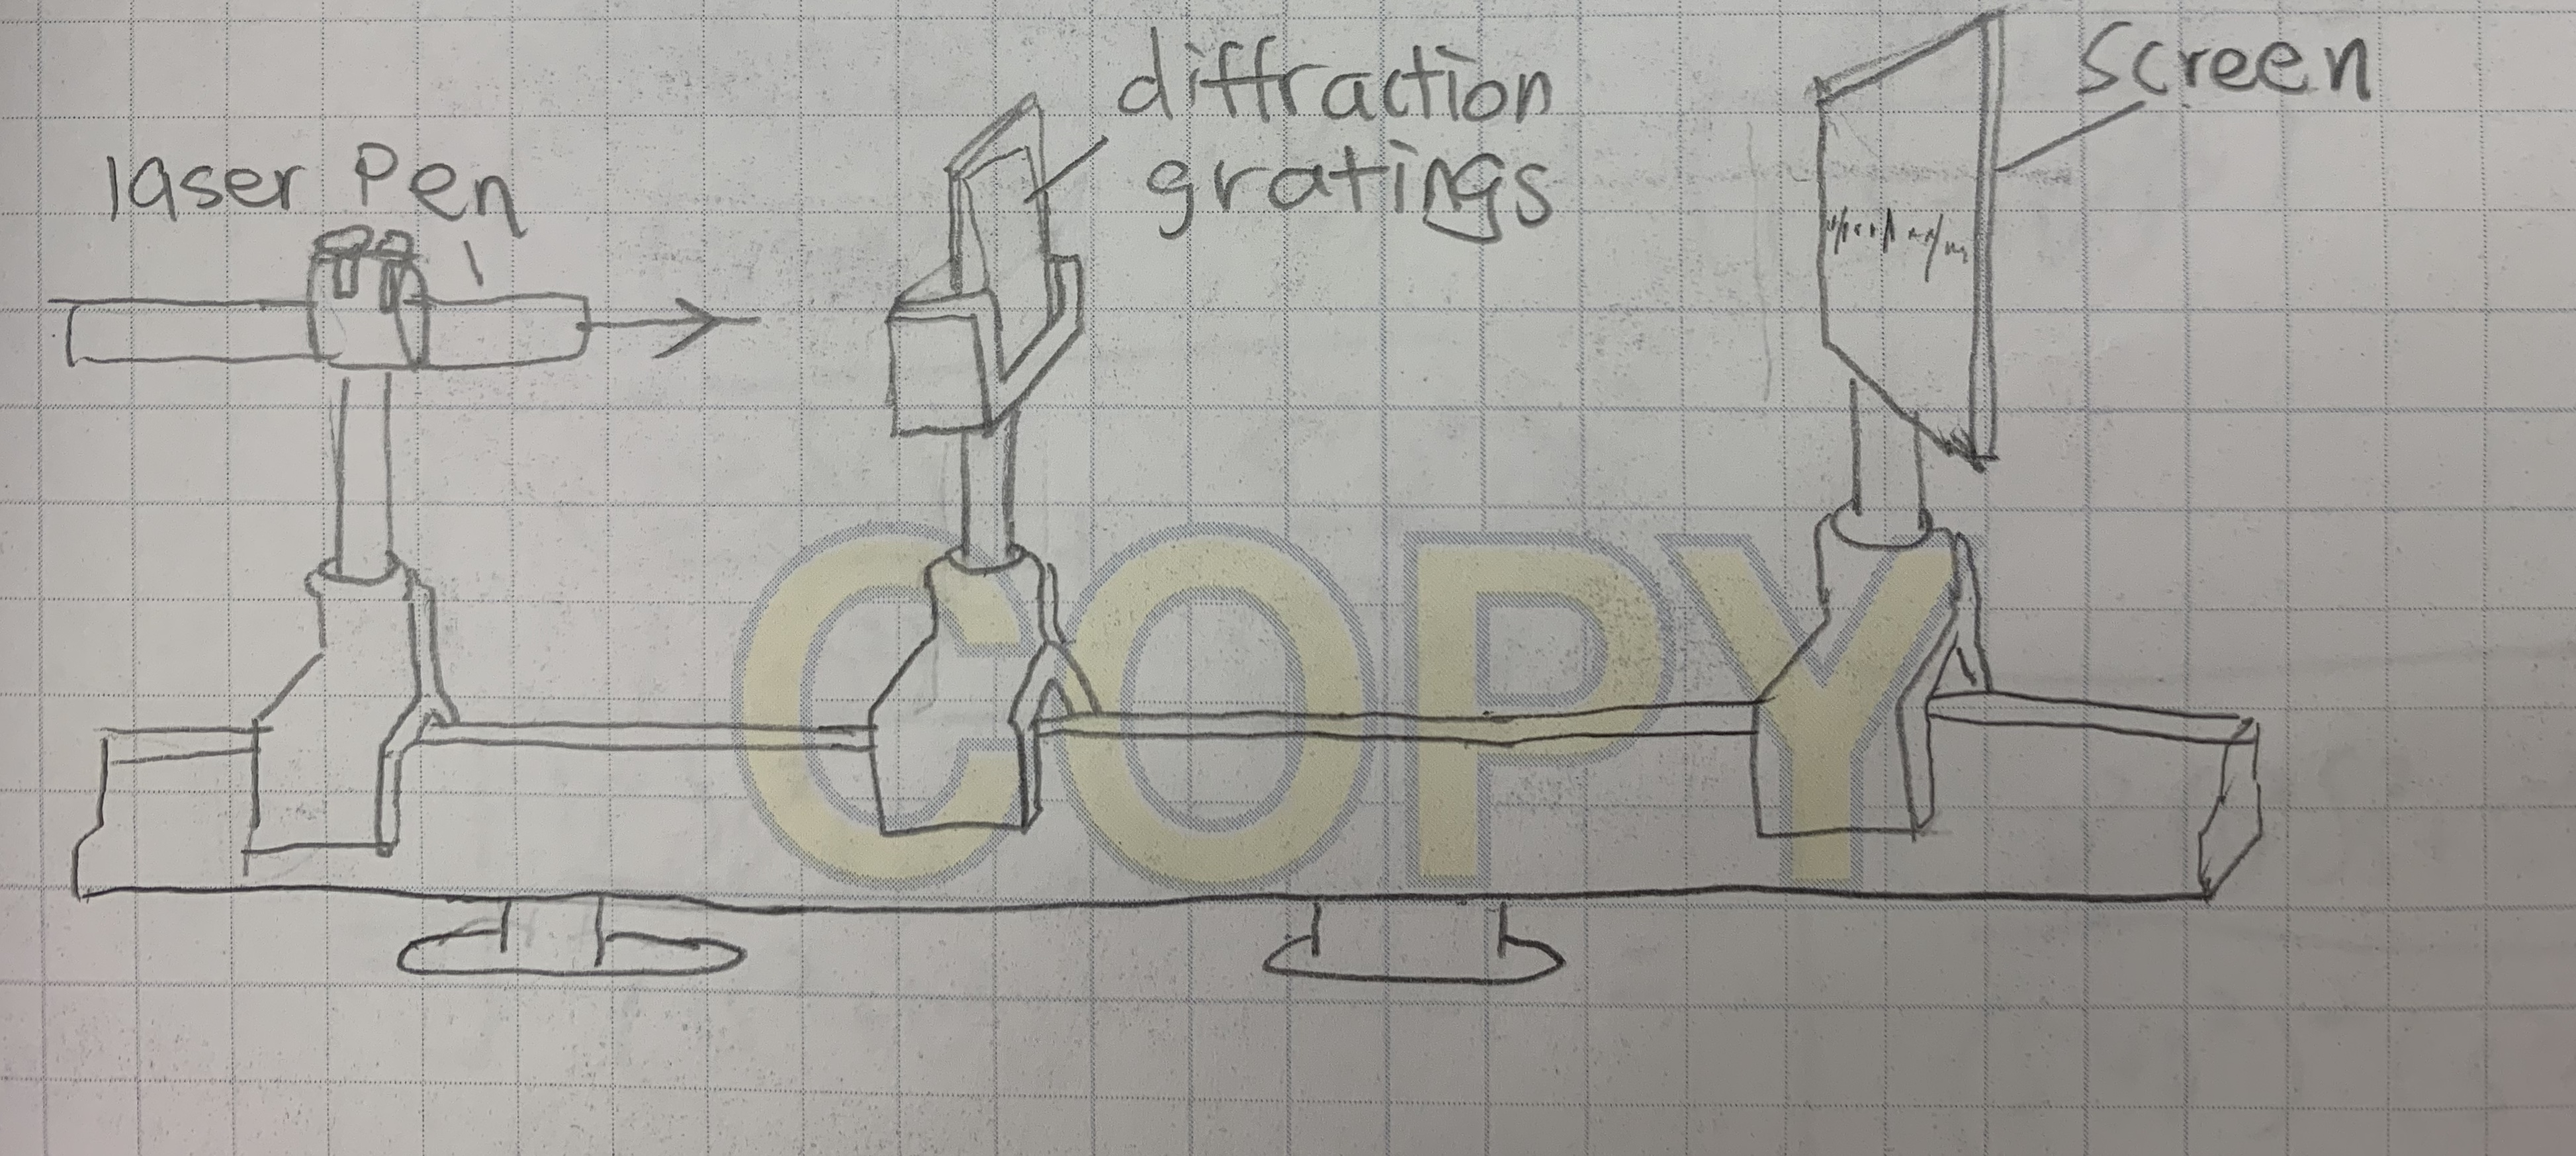
\includegraphics{fig1.jpg}
\caption{Experiment 4}
\end{figure}

    Note that in the following analysis, we let the variable \(a\) equal the
distance between the diffraction grating and the screen, and we let the
variable \(b\) represent the distance between the central maximum and
first fringe of the diffraction pattern on the screen. So then, to
collect data, we simply found \(a\) and \(b\) using first the violet
laser, and then the green laser, and then we used the following
equations.

From theory we know that if \(\theta\) is the angle between the central
maximum and the first fringe, \(d\) is the slit width of the diffraction
grating, and \(\lambda\) is the wavelength of the light being used, we
have:

\[\lambda = d\sin(\theta) \]

We also know that based on how the variables were defined,

\[ \theta = \arctan \left(\frac{a}{b}\right) \implies \lambda = \frac{da}{\sqrt{a^2 + b^2}}\]

If we finally note that in terms of the slight density \(D\),
\(d = \frac{1}{D}\), we have:

\[\lambda = \frac{a}{D\sqrt{a^2 + b^2}}\]

and therefore,

\[\delta\lambda = \sqrt{\dfrac{\left((a^{3} + b^{2}a)\frac{\delta D}{D}\right)^{2} + (b^{2}\delta a)^{2} + (ab\delta b)^{2}}{D^{2}(a^{2}+b^{2})^{3}}}\]

To find the corresponding frequencies of each laser, we simply used:

\[ f= \frac{c}{\lambda}\]

and,

\[ \delta f = \frac{c \: \delta\lambda}{\lambda^2}\]

Finally, it should be noted that in Experiment 1, we measured the slit
density \(D\) to be \(D = 5233 \pm 49 \; slits \cdot cm^{-1}\).

    \hypertarget{measuring-stopping-voltage-of-each-laser}{%
\subsubsection{Measuring stopping voltage of each
laser}\label{measuring-stopping-voltage-of-each-laser}}

To measure the stopping voltage, we first setup the circuit as indicated
in the figure below 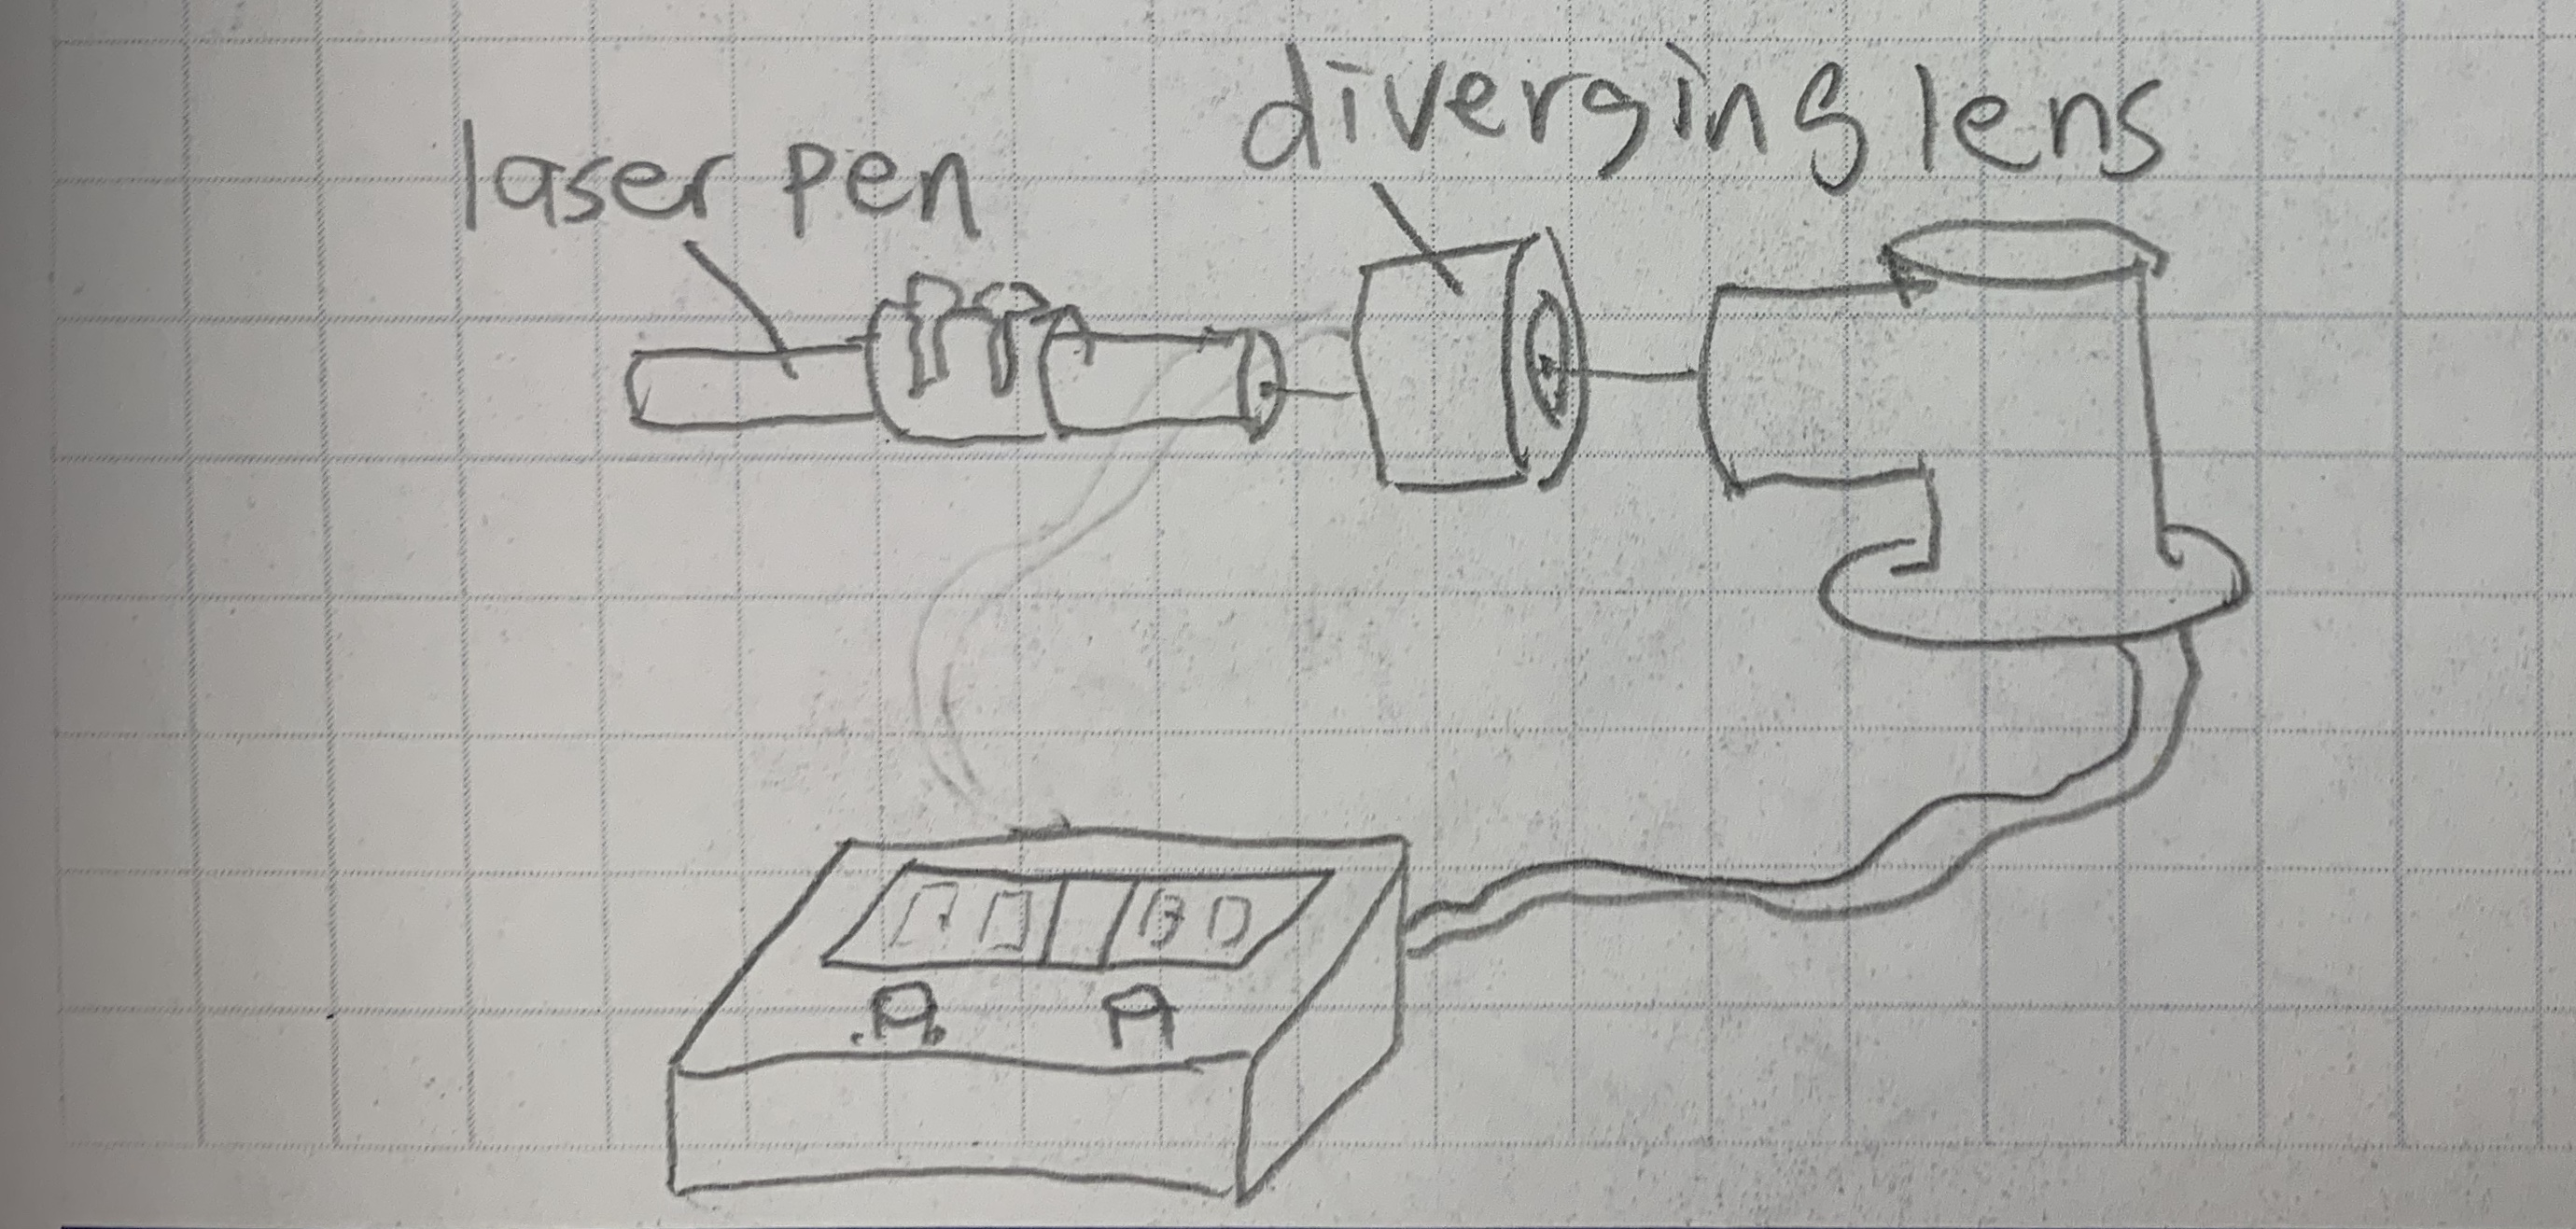
\includegraphics{fig2.jpg}

To calibrate the phototube, we simple covered the lid of the phototube
and pressed the calibration button for 5 seconds. We then shined the
laser pen through a diverging lens to disperse the light and ensure that
the photodiode was properly illuminated. Noting from the previous
experiment that the ``Photocurrent vs.~Voltage'' curve was not a linear
relationship, we simply decreased the voltage of the apparatus until the
photocurrent went to zero. By noting the fluctuations in the reading we
were able to determine the uncertainty in each measurement. As in the
previous experiment, we have:

\[eV_{stop} = hf - \phi\]

So the, finding \(h\) and \(\phi\) just becomes a matter of fitting our
data for \$eV\_\{stop\} \$ and \(f\) to a linear hypothesis and reading
off the regression parameters \(\hat{m}\) and \(\hat{b}\).

    \hypertarget{data-analysis}{%
\subsection{Data Analysis}\label{data-analysis}}

The wavelength of red laser is given to be: \[\lambda_{red}=634.6nm\]

For the violet laser, we measured \(b_{v}=24.2\pm0.05cm\) and
\(a_{v}=5.0\pm0.05cm\). Using the equations in the Method section, we
therefore determined:

\[\lambda_{violet} = 387\pm5.24nm\]

For the green laser, we measured \(b_{g}=21.7\pm0.05cm\) and
\(a_{g}=6.0\pm0.05cm\). Using the same equations, we determined:

\[\lambda_{green} = 510\pm6.28nm\]

After taking all the data, we have the following data table. Here
``Vstop'' and ``DeltaV'' denote the stopping voltage and its associated
uncertainty respectively, with units of mV, and lambda and DeltaLambda
denotes the wavelength of light and its associated uncertainty
respectively, with unit of nm.

    \begin{tcolorbox}[breakable, size=fbox, boxrule=1pt, pad at break*=1mm,colback=cellbackground, colframe=cellborder]
\prompt{In}{incolor}{4}{\hspace{4pt}}
\begin{Verbatim}[commandchars=\\\{\}]
\PY{n}{data4} \PY{o}{=} \PY{n}{pd}\PY{o}{.}\PY{n}{DataFrame}\PY{p}{(}\PY{p}{\PYZob{}}\PY{l+s+s1}{\PYZsq{}}\PY{l+s+s1}{Color}\PY{l+s+s1}{\PYZsq{}}\PY{p}{:}\PY{p}{[}\PY{l+s+s1}{\PYZsq{}}\PY{l+s+s1}{red}\PY{l+s+s1}{\PYZsq{}}\PY{p}{,} \PY{l+s+s1}{\PYZsq{}}\PY{l+s+s1}{green}\PY{l+s+s1}{\PYZsq{}}\PY{p}{,} \PY{l+s+s1}{\PYZsq{}}\PY{l+s+s1}{violet}\PY{l+s+s1}{\PYZsq{}}\PY{p}{]}\PY{p}{,} 
                      \PY{l+s+s1}{\PYZsq{}}\PY{l+s+s1}{Vstop}\PY{l+s+s1}{\PYZsq{}}\PY{p}{:}\PY{p}{[}\PY{o}{\PYZhy{}}\PY{l+m+mi}{314}\PY{p}{,} \PY{o}{\PYZhy{}}\PY{l+m+mi}{609}\PY{p}{,} \PY{o}{\PYZhy{}}\PY{l+m+mi}{1240}\PY{p}{]}\PY{p}{,} 
                      \PY{l+s+s1}{\PYZsq{}}\PY{l+s+s1}{DeltaV}\PY{l+s+s1}{\PYZsq{}}\PY{p}{:}\PY{p}{[}\PY{l+m+mi}{2}\PY{p}{,} \PY{l+m+mi}{2}\PY{p}{,} \PY{l+m+mi}{2}\PY{p}{]}\PY{p}{,} 
                      \PY{l+s+s1}{\PYZsq{}}\PY{l+s+s1}{lambda}\PY{l+s+s1}{\PYZsq{}}\PY{p}{:}\PY{p}{[}\PY{l+m+mf}{634.6}\PY{p}{,} \PY{l+m+mi}{510}\PY{p}{,} \PY{l+m+mi}{387}\PY{p}{]}\PY{p}{,} 
                      \PY{l+s+s1}{\PYZsq{}}\PY{l+s+s1}{DeltaLambda}\PY{l+s+s1}{\PYZsq{}}\PY{p}{:} \PY{p}{[}\PY{l+m+mi}{0}\PY{p}{,} \PY{l+m+mf}{6.28}\PY{p}{,} \PY{l+m+mf}{5.24}\PY{p}{]}\PY{p}{\PYZcb{}}\PY{p}{)}
\PY{n}{data4}
\end{Verbatim}
\end{tcolorbox}

            \begin{tcolorbox}[breakable, boxrule=.5pt, size=fbox, pad at break*=1mm, opacityfill=0]
\prompt{Out}{outcolor}{4}{\hspace{3.5pt}}
\begin{Verbatim}[commandchars=\\\{\}]
    Color  Vstop  DeltaV  lambda  DeltaLambda
0     red   -314       2   634.6         0.00
1   green   -609       2   510.0         6.28
2  violet  -1240       2   387.0         5.24
\end{Verbatim}
\end{tcolorbox}
        
    We would like \(K_{max}\) in terms of \(f\), so this following data
takes the above data, and uses the equation in the Method section to
find the desired quantities. In this data table, Kmax and DeltaKmax
denotes the maximum kinetic energy of photoelectron and its associated
uncertainty respectively, with units of eV, and f and Deltaf denotes the
incident laser frequency and its associated uncertainty respectively,
with unit of Hz.

    \begin{tcolorbox}[breakable, size=fbox, boxrule=1pt, pad at break*=1mm,colback=cellbackground, colframe=cellborder]
\prompt{In}{incolor}{7}{\hspace{4pt}}
\begin{Verbatim}[commandchars=\\\{\}]
\PY{n}{fit4} \PY{o}{=} \PY{n}{pd}\PY{o}{.}\PY{n}{DataFrame}\PY{p}{(}\PY{p}{)}
\PY{n}{fit4}\PY{p}{[}\PY{l+s+s1}{\PYZsq{}}\PY{l+s+s1}{f}\PY{l+s+s1}{\PYZsq{}}\PY{p}{]} \PY{o}{=} \PY{p}{(}\PY{l+m+mi}{3} \PY{o}{*} \PY{l+m+mi}{10}\PY{o}{*}\PY{o}{*}\PY{l+m+mi}{17}\PY{p}{)}\PY{o}{/}\PY{n}{data4}\PY{p}{[}\PY{l+s+s1}{\PYZsq{}}\PY{l+s+s1}{lambda}\PY{l+s+s1}{\PYZsq{}}\PY{p}{]}
\PY{n}{fit4}\PY{p}{[}\PY{l+s+s1}{\PYZsq{}}\PY{l+s+s1}{Deltaf}\PY{l+s+s1}{\PYZsq{}}\PY{p}{]} \PY{o}{=} \PY{o}{\PYZhy{}}\PY{p}{(}\PY{l+m+mi}{3} \PY{o}{*} \PY{l+m+mi}{10}\PY{o}{*}\PY{o}{*}\PY{l+m+mi}{17}\PY{p}{)} \PY{o}{*} \PY{n}{data4}\PY{p}{[}\PY{l+s+s1}{\PYZsq{}}\PY{l+s+s1}{DeltaLambda}\PY{l+s+s1}{\PYZsq{}}\PY{p}{]}\PY{o}{/}\PY{n}{data4}\PY{p}{[}\PY{l+s+s1}{\PYZsq{}}\PY{l+s+s1}{lambda}\PY{l+s+s1}{\PYZsq{}}\PY{p}{]}\PY{o}{*}\PY{o}{*}\PY{l+m+mi}{2}
\PY{n}{fit4}\PY{p}{[}\PY{l+s+s1}{\PYZsq{}}\PY{l+s+s1}{Kmax}\PY{l+s+s1}{\PYZsq{}}\PY{p}{]} \PY{o}{=} \PY{o}{\PYZhy{}}\PY{n}{data4}\PY{p}{[}\PY{l+s+s1}{\PYZsq{}}\PY{l+s+s1}{Vstop}\PY{l+s+s1}{\PYZsq{}}\PY{p}{]}\PY{o}{*}\PY{l+m+mi}{10}\PY{o}{*}\PY{o}{*}\PY{o}{\PYZhy{}}\PY{l+m+mi}{3}
\PY{n}{fit4}\PY{p}{[}\PY{l+s+s1}{\PYZsq{}}\PY{l+s+s1}{DeltaKmax}\PY{l+s+s1}{\PYZsq{}}\PY{p}{]} \PY{o}{=} \PY{n}{data4}\PY{p}{[}\PY{l+s+s1}{\PYZsq{}}\PY{l+s+s1}{DeltaV}\PY{l+s+s1}{\PYZsq{}}\PY{p}{]}\PY{o}{*}\PY{l+m+mi}{10}\PY{o}{*}\PY{o}{*}\PY{o}{\PYZhy{}}\PY{l+m+mi}{3}
\PY{n}{fit4}
\end{Verbatim}
\end{tcolorbox}

            \begin{tcolorbox}[breakable, boxrule=.5pt, size=fbox, pad at break*=1mm, opacityfill=0]
\prompt{Out}{outcolor}{7}{\hspace{3.5pt}}
\begin{Verbatim}[commandchars=\\\{\}]
              f        Deltaf   Kmax  DeltaKmax
0  4.727387e+14 -0.000000e+00  0.314      0.002
1  5.882353e+14 -7.243368e+12  0.609      0.002
2  7.751938e+14 -1.049616e+13  1.240      0.002
\end{Verbatim}
\end{tcolorbox}
        
    The following plot gives a visual of this data with its associated
uncertainties:

    \begin{tcolorbox}[breakable, size=fbox, boxrule=1pt, pad at break*=1mm,colback=cellbackground, colframe=cellborder]
\prompt{In}{incolor}{10}{\hspace{4pt}}
\begin{Verbatim}[commandchars=\\\{\}]
\PY{n}{plt}\PY{o}{.}\PY{n}{errorbar}\PY{p}{(}\PY{n}{fit4}\PY{o}{.}\PY{n}{f}\PY{p}{,} \PY{n}{fit4}\PY{o}{.}\PY{n}{Kmax}\PY{p}{,} \PY{n}{yerr}\PY{o}{=}\PY{n}{fit4}\PY{o}{.}\PY{n}{DeltaKmax}\PY{p}{,} \PY{n}{xerr}\PY{o}{=}\PY{n}{fit4}\PY{o}{.}\PY{n}{Deltaf}\PY{p}{,} \PY{n}{fmt}\PY{o}{=}\PY{l+s+s1}{\PYZsq{}}\PY{l+s+s1}{.}\PY{l+s+s1}{\PYZsq{}}\PY{p}{)}
\PY{n}{plt}\PY{o}{.}\PY{n}{xlabel}\PY{p}{(}\PY{l+s+s2}{\PYZdq{}}\PY{l+s+s2}{Frequency (Hz)}\PY{l+s+s2}{\PYZdq{}}\PY{p}{)}
\PY{n}{plt}\PY{o}{.}\PY{n}{ylabel}\PY{p}{(}\PY{l+s+s2}{\PYZdq{}}\PY{l+s+s2}{K Max (eV)}\PY{l+s+s2}{\PYZdq{}}\PY{p}{)}
\PY{n}{plt}\PY{o}{.}\PY{n}{title}\PY{p}{(}\PY{l+s+s2}{\PYZdq{}}\PY{l+s+s2}{K Max vs. Frequency}\PY{l+s+s2}{\PYZdq{}}\PY{p}{)}
\PY{n}{plt}\PY{o}{.}\PY{n}{grid}\PY{p}{(}\PY{p}{)}
\end{Verbatim}
\end{tcolorbox}

    \begin{center}
    \adjustimage{max size={0.9\linewidth}{0.9\paperheight}}{output_26_0.png}
    \end{center}
    { \hspace*{\fill} \\}
    
    Note that the error bars are very small and difficult to see. Now that
we have our data in the appropriate format, we used a weighted
least-squares fit to fit our data to a linear hypothesis
\(K_{max} = \hat{m}f + \hat{b}\), noting that \(h = \hat{m}\) and
\(\phi = -\hat{b}\). The script used to find the best fit parameters was
quite long, and is therefore included in the References section. After
fitting the data, we found that:


$$h = \hat{m} = (2.94 \pm 0.094) \times 10^{-15}\;eVs $$
$$\phi = -\hat{b}= 1.08\pm0.04 \;eV$$


    The accepted values for these two quantities is
\(h = 4.136 \times 10^{-15} eV\cdot s\) and \(\phi = 1.911 eV\). Simple
agreement tests between our data and the accepted values yield 6.3 for
\(h\) and 10.4 for \(\phi\). Therefore we see that the values predicted
by our data do not agree with accepted values. I believe that the reason
these values do not agree is because our values of uncertainty for
\(V_{stop}\) were too small. To measure these uncertainties, we simply
measured the fluctuations in the measurement device, but based on the
data we took in Experiment 3, it is likely that we did not properly
determine the range of voltages over which \(V_{stop}\) was nearly zero,
which would have given us a larger uncertainty in our measurement, and
may have caused the values we received in our analysis to agree with
accepted values.

    \hypertarget{experiment-5---photocurrent-vs.-intensity}{%
\section{Experiment 5 - Photocurrent
vs.~Intensity}\label{experiment-5---photocurrent-vs.-intensity}}

\hypertarget{objective}{%
\subsection{Objective:}\label{objective}}

The purpose of this experiment is to determine how the photocurrent of
the photoelectric effect apparatus depends on the intensity of the
incident light.

\hypertarget{method-and-experimental-procedure}{%
\subsection{Method and Experimental
Procedure:}\label{method-and-experimental-procedure}}

We first set up the photoelectric effect apparatus according to the
section ``The Photoelectric Effect Setup'' in the lab manual. We then
calibrated the apparatus using the procedure specified in the lab
manual, which basically entails covering the phototube, and then pushing
the calibration button for 5 seconds.

We decided to only use the blue and the green LEDs for this experiment.
We were trying to determine the relationship between the Photocurrent
and the and Intensity of the incident light, and so for a given LED, we
set the voltage of the apparatus to 0 and varied the power of the LED
and measured the Photocurrent.

After taking this data, we had a relationship between Power (L0xx) and
the Photocurrent, and then we used the data tables provided to us by the
lab instructor to convert between Power (L0xx) and Intensity. This
allowed us to make the data tables and graphs we needed which show the
relationship between Intensity and Photocurrent.

    \hypertarget{data-analysis}{%
\subsection{Data Analysis:}\label{data-analysis}}

The following data tables show the data we took for each LED in this
experiment. Here ``Power'' is measured in L0xx, ``Intensity'' is
measured in Lux, and ``Photocurrent'' is measured in milliamps.
``Delta\_PC'' represents the corresponding measurement uncertainty in
Photocurrent.

Green Data:

    \begin{tcolorbox}[breakable, size=fbox, boxrule=1pt, pad at break*=1mm,colback=cellbackground, colframe=cellborder]
\prompt{In}{incolor}{22}{\hspace{4pt}}
\begin{Verbatim}[commandchars=\\\{\}]
\PY{n}{green5}
\end{Verbatim}
\end{tcolorbox}

            \begin{tcolorbox}[breakable, boxrule=.5pt, size=fbox, pad at break*=1mm, opacityfill=0]
\prompt{Out}{outcolor}{22}{\hspace{3.5pt}}
\begin{Verbatim}[commandchars=\\\{\}]
   Power  Intensity  Photocurrent  Delta\_PC
0     15         26            19         2
1     19       4200           550         2
2     26      25800          1602         2
3     30      41100          2018         2
4     35      55900          2345         2
5     39      70200          2610         2
\end{Verbatim}
\end{tcolorbox}
        
    Blue Data:

    \begin{tcolorbox}[breakable, size=fbox, boxrule=1pt, pad at break*=1mm,colback=cellbackground, colframe=cellborder]
\prompt{In}{incolor}{23}{\hspace{4pt}}
\begin{Verbatim}[commandchars=\\\{\}]
\PY{n}{blue5}
\end{Verbatim}
\end{tcolorbox}

            \begin{tcolorbox}[breakable, boxrule=.5pt, size=fbox, pad at break*=1mm, opacityfill=0]
\prompt{Out}{outcolor}{23}{\hspace{3.5pt}}
\begin{Verbatim}[commandchars=\\\{\}]
   Power  Intensity  Photocurrent  Delta\_PC
0     18       1980           553         2
1     24      25500          3428         2
2     28      51300          4884         2
3     30      64600          5484         2
4     33      81000          6012         2
5     37     106000          6904         2
\end{Verbatim}
\end{tcolorbox}
        
    The following graphs plot the Photocurrent versus the Intensity for each
LED, with error bars. Note that the error bars are basically impossible
to see because they are so small.

Green Graph:

    \begin{tcolorbox}[breakable, size=fbox, boxrule=1pt, pad at break*=1mm,colback=cellbackground, colframe=cellborder]
\prompt{In}{incolor}{28}{\hspace{4pt}}
\begin{Verbatim}[commandchars=\\\{\}]
\PY{n}{plt}\PY{o}{.}\PY{n}{errorbar}\PY{p}{(}\PY{n}{green5}\PY{o}{.}\PY{n}{Intensity}\PY{p}{,} \PY{n}{green5}\PY{o}{.}\PY{n}{Photocurrent}\PY{p}{,} \PY{n}{yerr}\PY{o}{=}\PY{n}{green5}\PY{o}{.}\PY{n}{Delta\PYZus{}PC}\PY{p}{)}
\PY{n}{plt}\PY{o}{.}\PY{n}{title}\PY{p}{(}\PY{l+s+s2}{\PYZdq{}}\PY{l+s+s2}{Photocurrent vs. Intensity (Green)}\PY{l+s+s2}{\PYZdq{}}\PY{p}{)}
\PY{n}{plt}\PY{o}{.}\PY{n}{xlabel}\PY{p}{(}\PY{l+s+s2}{\PYZdq{}}\PY{l+s+s2}{Intensity (Lux)}\PY{l+s+s2}{\PYZdq{}}\PY{p}{)}
\PY{n}{plt}\PY{o}{.}\PY{n}{ylabel}\PY{p}{(}\PY{l+s+s2}{\PYZdq{}}\PY{l+s+s2}{Photocurrent (mA)}\PY{l+s+s2}{\PYZdq{}}\PY{p}{)}
\PY{n}{plt}\PY{o}{.}\PY{n}{show}\PY{p}{(}\PY{p}{)}
\end{Verbatim}
\end{tcolorbox}

    \begin{center}
    \adjustimage{max size={0.9\linewidth}{0.9\paperheight}}{output_35_0.png}
    \end{center}
    { \hspace*{\fill} \\}
    
    Blue Graph:

    \begin{tcolorbox}[breakable, size=fbox, boxrule=1pt, pad at break*=1mm,colback=cellbackground, colframe=cellborder]
\prompt{In}{incolor}{29}{\hspace{4pt}}
\begin{Verbatim}[commandchars=\\\{\}]
\PY{n}{plt}\PY{o}{.}\PY{n}{errorbar}\PY{p}{(}\PY{n}{blue5}\PY{o}{.}\PY{n}{Intensity}\PY{p}{,} \PY{n}{blue5}\PY{o}{.}\PY{n}{Photocurrent}\PY{p}{,} \PY{n}{yerr}\PY{o}{=}\PY{n}{blue5}\PY{o}{.}\PY{n}{Delta\PYZus{}PC}\PY{p}{)}
\PY{n}{plt}\PY{o}{.}\PY{n}{title}\PY{p}{(}\PY{l+s+s2}{\PYZdq{}}\PY{l+s+s2}{Photocurrent vs. Intensity (Blue)}\PY{l+s+s2}{\PYZdq{}}\PY{p}{)}
\PY{n}{plt}\PY{o}{.}\PY{n}{xlabel}\PY{p}{(}\PY{l+s+s2}{\PYZdq{}}\PY{l+s+s2}{Intensity (Lux)}\PY{l+s+s2}{\PYZdq{}}\PY{p}{)}
\PY{n}{plt}\PY{o}{.}\PY{n}{ylabel}\PY{p}{(}\PY{l+s+s2}{\PYZdq{}}\PY{l+s+s2}{Photocurrent (mA)}\PY{l+s+s2}{\PYZdq{}}\PY{p}{)}
\PY{n}{plt}\PY{o}{.}\PY{n}{show}\PY{p}{(}\PY{p}{)}
\end{Verbatim}
\end{tcolorbox}

    \begin{center}
    \adjustimage{max size={0.9\linewidth}{0.9\paperheight}}{output_37_0.png}
    \end{center}
    { \hspace*{\fill} \\}
    
    The quantum mechanical description of this experiment relies on
knowledge of the geometry of the photocurrent apparatus, which we do not
possess, and it would be quite complicated even if we did. Because of
this, we do not have a good idea of a hypothesis to which we should
attempt to fit our data. Therefore I will provide a qualitative analysis
of the above graphs and provide explanations for their behavior.

Both of the above graphs are characterized by a positive first
derivative, and a negative second derivative. To explain this behavior
using quantum theory, we note that light is quantized into individual
packets of energy called photons, each with an energy \(hf\). Every time
a photon is absorbed by an electron in the semi-conducting material,
that electron gains the energy in the photon, and if the energy absorbed
is greater than the work function of the material, the electron will be
freed from the material, and we will measure it as Photocurrent. So
then, increasing the intensity of the light source can be interpreted as
increasing the rate at which the light source emits photons. However,
because there is only a finite number of electrons in the material, the
greater number of photons will have a harder time finding electrons that
have not already absorbed a photon (this is a very hand-wavy argument,
but it is sufficiently correct for this explanation). Therefore
increasing the intensity of light will increase the photocurrent, but
the rate at which the photocurrent increases will decrease as the
intensity increases.

We therefore see that our data supports the viewpoint that light is
quantized, because our graphs show a positive first derivative, and a
negative second derivative.

    \hypertarget{summary-and-conclusion}{%
\section{Summary and Conclusion}\label{summary-and-conclusion}}

In this lab we were supposed to explore the photoelectric effect,
observe the properties of the experiment that support the particle
nature of light, and learn how to determine Plancks' constant.

Experiments 3, 4, and 5 allowed us to explore the photoelectric effect
and observe the particle nature of light, and in Experiments 3 and 4 we
found Planck's constant. We therefore met all of the overall objectives
of this lab.

In Lab 3, we were supposed to determine Planck's constant, and the
cutoff frequency and work function of the semi-conducting material in
the photodiode using the LEDs provided to us. The values we found in
this experiment agreed with the accepted values posted in the lab
manual.

In Lab 4, the objective was the same as Lab3, but we were supposed to
use lasers instead of LEDs to minimize uncertainty in measurements of
wavelength of incident light. The values we found did not agree with the
accepted values, and as is explained further in the Data Analysis
section of its report, I believe this disagreement is due to the fact
that we did not properly measure the uncertainty in our readings of the
stopping voltage.

In Lab 5, the objective was to find the relationship between the
intensity of the incident light and the photocurrent of the
photoelectric effect apparatus. We found that the curve of photocurrent
as a function of intensity is characterized by a positive first
derivative, and a negative second derivative, and as is explained
further in the Data Analysis section of that experiment, this behavior
supports the particle nature of light.

    \hypertarget{contributions}{%
\section{Contributions}\label{contributions}}

Danny and Heidi did equal shares of the lab work and data analysis, and
Danny did 65\% of the work writing the interpretations of the data
analysis.

    \hypertarget{references}{%
\section{References}\label{references}}

We used python and the open source python libraries Pandas, Matplotlib,
SciPy, and Numpy.

    \begin{tcolorbox}[breakable, size=fbox, boxrule=1pt, pad at break*=1mm,colback=cellbackground, colframe=cellborder]
\prompt{In}{incolor}{17}{\hspace{4pt}}
\begin{Verbatim}[commandchars=\\\{\}]
\PY{k+kn}{import} \PY{n+nn}{pandas} \PY{k}{as} \PY{n+nn}{pd} 
\PY{k+kn}{import} \PY{n+nn}{matplotlib}\PY{n+nn}{.}\PY{n+nn}{pyplot} \PY{k}{as} \PY{n+nn}{plt}
\PY{k+kn}{from} \PY{n+nn}{math} \PY{k}{import} \PY{o}{*}
\PY{k+kn}{from} \PY{n+nn}{scipy} \PY{k}{import} \PY{n}{stats}
\PY{k+kn}{import} \PY{n+nn}{numpy} \PY{k}{as} \PY{n+nn}{np}
\PY{k+kn}{from} \PY{n+nn}{IPython}\PY{n+nn}{.}\PY{n+nn}{display} \PY{k}{import} \PY{n}{Image}
\PY{n}{im2} \PY{o}{=} \PY{n}{Image}\PY{p}{(}\PY{l+s+s1}{\PYZsq{}}\PY{l+s+s1}{fig2.jpg}\PY{l+s+s1}{\PYZsq{}}\PY{p}{)}
\PY{n}{im1} \PY{o}{=} \PY{n}{Image}\PY{p}{(}\PY{l+s+s1}{\PYZsq{}}\PY{l+s+s1}{fig1.jpg}\PY{l+s+s1}{\PYZsq{}}\PY{p}{)}
\end{Verbatim}
\end{tcolorbox}

    The following scripts were used to generate data tables in experiment 3.

    \begin{tcolorbox}[breakable, size=fbox, boxrule=1pt, pad at break*=1mm,colback=cellbackground, colframe=cellborder]
\prompt{In}{incolor}{60}{\hspace{4pt}}
\begin{Verbatim}[commandchars=\\\{\}]
\PY{n}{blue} \PY{o}{=} \PY{n}{pd}\PY{o}{.}\PY{n}{DataFrame}\PY{p}{(}\PY{p}{\PYZob{}}\PY{l+s+s2}{\PYZdq{}}\PY{l+s+s2}{V}\PY{l+s+s2}{\PYZdq{}}\PY{p}{:} 
                     \PY{p}{[}\PY{o}{\PYZhy{}}\PY{l+m+mi}{931}\PY{p}{,} \PY{o}{\PYZhy{}}\PY{l+m+mi}{800}\PY{p}{,} \PY{o}{\PYZhy{}}\PY{l+m+mi}{700}\PY{p}{,} \PY{o}{\PYZhy{}}\PY{l+m+mi}{600}\PY{p}{,} \PY{o}{\PYZhy{}}\PY{l+m+mi}{500}\PY{p}{,} \PY{o}{\PYZhy{}}\PY{l+m+mi}{300}\PY{p}{,} \PY{o}{\PYZhy{}}\PY{l+m+mi}{100}\PY{p}{,} \PY{l+m+mi}{0}\PY{p}{,} \PY{l+m+mi}{200}\PY{p}{,} \PY{l+m+mi}{400}\PY{p}{]}\PY{p}{,}
                    \PY{l+s+s2}{\PYZdq{}}\PY{l+s+s2}{Photocurrent}\PY{l+s+s2}{\PYZdq{}}\PY{p}{:}
                    \PY{p}{[}\PY{l+m+mi}{0}\PY{p}{,} \PY{l+m+mi}{114}\PY{p}{,} \PY{l+m+mi}{321}\PY{p}{,} \PY{l+m+mi}{680}\PY{p}{,} \PY{l+m+mi}{1194}\PY{p}{,} \PY{l+m+mi}{2661}\PY{p}{,} \PY{l+m+mi}{4563}\PY{p}{,} \PY{l+m+mi}{5598}\PY{p}{,} \PY{l+m+mi}{7684}\PY{p}{,} \PY{l+m+mi}{9779}\PY{p}{]}\PY{p}{,}
                    \PY{l+s+s2}{\PYZdq{}}\PY{l+s+s2}{delta\PYZus{}pc}\PY{l+s+s2}{\PYZdq{}}\PY{p}{:}
                    \PY{p}{[}\PY{l+m+mi}{1}\PY{p}{,} \PY{l+m+mi}{2}\PY{p}{,} \PY{l+m+mi}{2}\PY{p}{,} \PY{l+m+mi}{2}\PY{p}{,} \PY{l+m+mi}{2}\PY{p}{,} \PY{l+m+mi}{2}\PY{p}{,} \PY{l+m+mi}{2}\PY{p}{,} \PY{l+m+mi}{2}\PY{p}{,} \PY{l+m+mi}{3}\PY{p}{,} \PY{l+m+mi}{2}\PY{p}{]}\PY{p}{\PYZcb{}}\PY{p}{)}

\PY{n}{green} \PY{o}{=} \PY{n}{pd}\PY{o}{.}\PY{n}{DataFrame}\PY{p}{(}\PY{p}{\PYZob{}}\PY{l+s+s2}{\PYZdq{}}\PY{l+s+s2}{V}\PY{l+s+s2}{\PYZdq{}}\PY{p}{:}
                     \PY{p}{[}\PY{o}{\PYZhy{}}\PY{l+m+mi}{750}\PY{p}{,} \PY{o}{\PYZhy{}}\PY{l+m+mi}{600}\PY{p}{,} \PY{o}{\PYZhy{}}\PY{l+m+mi}{400}\PY{p}{,} \PY{o}{\PYZhy{}}\PY{l+m+mi}{200}\PY{p}{,} \PY{l+m+mi}{0}\PY{p}{,} \PY{l+m+mi}{100}\PY{p}{,} \PY{l+m+mi}{200}\PY{p}{,} \PY{l+m+mi}{300}\PY{p}{,} \PY{l+m+mi}{400}\PY{p}{]}\PY{p}{,}
                     \PY{l+s+s2}{\PYZdq{}}\PY{l+s+s2}{Photocurrent}\PY{l+s+s2}{\PYZdq{}}\PY{p}{:}
                     \PY{p}{[}\PY{l+m+mi}{0}\PY{p}{,} \PY{l+m+mi}{18}\PY{p}{,} \PY{l+m+mi}{223}\PY{p}{,} \PY{l+m+mi}{945}\PY{p}{,} \PY{l+m+mi}{2056}\PY{p}{,} \PY{l+m+mi}{2653}\PY{p}{,} \PY{l+m+mi}{3236}\PY{p}{,} \PY{l+m+mi}{3815}\PY{p}{,} \PY{l+m+mi}{4392}\PY{p}{]}\PY{p}{,}
                     \PY{l+s+s2}{\PYZdq{}}\PY{l+s+s2}{delta\PYZus{}pc}\PY{l+s+s2}{\PYZdq{}}\PY{p}{:}
                     \PY{p}{[}\PY{l+m+mi}{3}\PY{p}{,} \PY{l+m+mi}{3}\PY{p}{,} \PY{l+m+mi}{2}\PY{p}{,} \PY{l+m+mi}{2}\PY{p}{,} \PY{l+m+mi}{2}\PY{p}{,} \PY{l+m+mi}{2}\PY{p}{,} \PY{l+m+mi}{2}\PY{p}{,} \PY{l+m+mi}{2}\PY{p}{,} \PY{l+m+mi}{1}\PY{p}{]}\PY{p}{\PYZcb{}}\PY{p}{)}
\PY{n}{red} \PY{o}{=} \PY{n}{pd}\PY{o}{.}\PY{n}{DataFrame}\PY{p}{(}\PY{p}{\PYZob{}}\PY{l+s+s2}{\PYZdq{}}\PY{l+s+s2}{V}\PY{l+s+s2}{\PYZdq{}}\PY{p}{:}
                   \PY{p}{[}\PY{o}{\PYZhy{}}\PY{l+m+mi}{400}\PY{p}{,} \PY{o}{\PYZhy{}}\PY{l+m+mi}{300}\PY{p}{,} \PY{o}{\PYZhy{}}\PY{l+m+mi}{200}\PY{p}{,} \PY{o}{\PYZhy{}}\PY{l+m+mi}{100}\PY{p}{,} \PY{l+m+mi}{0}\PY{p}{,} \PY{l+m+mi}{100}\PY{p}{,} \PY{l+m+mi}{200}\PY{p}{,} \PY{l+m+mi}{300}\PY{p}{,} \PY{l+m+mi}{400}\PY{p}{]}\PY{p}{,}

                    \PY{l+s+s2}{\PYZdq{}}\PY{l+s+s2}{Photocurrent}\PY{l+s+s2}{\PYZdq{}}\PY{p}{:}
                   \PY{p}{[}\PY{l+m+mi}{0}\PY{p}{,} \PY{l+m+mi}{9}\PY{p}{,} \PY{l+m+mi}{28}\PY{p}{,} \PY{l+m+mi}{128}\PY{p}{,} \PY{l+m+mi}{392}\PY{p}{,} \PY{l+m+mi}{720}\PY{p}{,} \PY{l+m+mi}{1034}\PY{p}{,} \PY{l+m+mi}{1323}\PY{p}{,} \PY{l+m+mi}{1586}\PY{p}{]}\PY{p}{,}
                   \PY{l+s+s2}{\PYZdq{}}\PY{l+s+s2}{delta\PYZus{}pc}\PY{l+s+s2}{\PYZdq{}}\PY{p}{:}
                   \PY{p}{[}\PY{l+m+mi}{2}\PY{p}{,} \PY{l+m+mi}{2}\PY{p}{,} \PY{l+m+mi}{2}\PY{p}{,} \PY{l+m+mi}{2}\PY{p}{,} \PY{l+m+mi}{2}\PY{p}{,} \PY{l+m+mi}{2}\PY{p}{,} \PY{l+m+mi}{2}\PY{p}{,} \PY{l+m+mi}{2}\PY{p}{,} \PY{l+m+mi}{2}\PY{p}{]}\PY{p}{\PYZcb{}}\PY{p}{)}
\end{Verbatim}
\end{tcolorbox}

    \begin{tcolorbox}[breakable, size=fbox, boxrule=1pt, pad at break*=1mm,colback=cellbackground, colframe=cellborder]
\prompt{In}{incolor}{41}{\hspace{4pt}}
\begin{Verbatim}[commandchars=\\\{\}]
\PY{n}{data3} \PY{o}{=} \PY{n}{pd}\PY{o}{.}\PY{n}{DataFrame}\PY{p}{(}\PY{p}{)}
\PY{n}{data3} \PY{o}{=} \PY{n}{pd}\PY{o}{.}\PY{n}{DataFrame}\PY{p}{(}\PY{p}{\PYZob{}}\PY{l+s+s2}{\PYZdq{}}\PY{l+s+s2}{f}\PY{l+s+s2}{\PYZdq{}}\PY{p}{:}
                      \PY{p}{[}\PY{l+m+mf}{6.50e14}\PY{p}{,} \PY{l+m+mf}{5.62e14}\PY{p}{,} \PY{l+m+mf}{4.85e14}\PY{p}{]}\PY{p}{,}
                      \PY{l+s+s1}{\PYZsq{}}\PY{l+s+s1}{df}\PY{l+s+s1}{\PYZsq{}}\PY{p}{:}
                      \PY{p}{[}\PY{l+m+mf}{5.90e13}\PY{p}{,} \PY{l+m+mf}{4.32e13}\PY{p}{,} \PY{l+m+mf}{3.30e13}\PY{p}{]}\PY{p}{,}
                     \PY{l+s+s2}{\PYZdq{}}\PY{l+s+s2}{K}\PY{l+s+s2}{\PYZdq{}}\PY{p}{:}
                     \PY{p}{[}\PY{o}{.}\PY{l+m+mi}{931}\PY{p}{,} \PY{o}{.}\PY{l+m+mi}{750}\PY{p}{,} \PY{o}{.}\PY{l+m+mi}{400}\PY{p}{]}\PY{p}{,}
                     \PY{l+s+s2}{\PYZdq{}}\PY{l+s+s2}{dK}\PY{l+s+s2}{\PYZdq{}}\PY{p}{:}
                     \PY{p}{[}\PY{l+m+mf}{0.0023}\PY{p}{,} \PY{l+m+mf}{0.017}\PY{p}{,} \PY{l+m+mf}{0.023}\PY{p}{]}\PY{p}{\PYZcb{}}\PY{p}{)}
\end{Verbatim}
\end{tcolorbox}

    The following scripts represent error propagation calculation to find
the uncertainty in slit density, the green laser wavelength, and the
violet laser wavelength.

    \begin{tcolorbox}[breakable, size=fbox, boxrule=1pt, pad at break*=1mm,colback=cellbackground, colframe=cellborder]
\prompt{In}{incolor}{104}{\hspace{4pt}}
\begin{Verbatim}[commandchars=\\\{\}]
\PY{c+c1}{\PYZsh{}propagating error of slit density}

\PY{n}{a} \PY{o}{=} \PY{l+m+mi}{5}
\PY{n}{b} \PY{o}{=} \PY{l+m+mf}{14.2}
\PY{n}{db} \PY{o}{=} \PY{l+m+mf}{0.05}
\PY{n}{da} \PY{o}{=} \PY{l+m+mf}{0.05}
\PY{n}{l} \PY{o}{=} \PY{l+m+mf}{6.346e\PYZhy{}5}
\PY{n}{dl} \PY{o}{=} \PY{l+m+mi}{0}
\PY{n}{dD} \PY{o}{=} \PY{n}{math}\PY{o}{.}\PY{n}{sqrt}\PY{p}{(}\PY{p}{(}\PY{p}{(}\PY{p}{(}\PY{p}{(}\PY{n}{a}\PY{o}{*}\PY{o}{*}\PY{l+m+mi}{3} \PY{o}{+} \PY{n}{a}\PY{o}{*}\PY{n}{b}\PY{o}{*}\PY{o}{*}\PY{l+m+mi}{2}\PY{p}{)}\PY{o}{*}\PY{n}{dl}\PY{o}{/}\PY{n}{l}\PY{p}{)}\PY{o}{*}\PY{o}{*}\PY{l+m+mi}{2} \PY{o}{+} \PY{p}{(}\PY{n}{b}\PY{o}{*}\PY{o}{*}\PY{l+m+mi}{2} \PY{o}{*} \PY{n}{da}\PY{p}{)}\PY{o}{*}\PY{o}{*}\PY{l+m+mi}{2} \PY{o}{+} \PY{p}{(}\PY{n}{a}\PY{o}{*}\PY{n}{b}\PY{o}{*}\PY{n}{db}\PY{p}{)}\PY{o}{*}\PY{o}{*}\PY{l+m+mi}{2}\PY{p}{)}\PY{p}{)} \PY{o}{/}\PY{p}{(}\PY{p}{(}\PY{n}{a}\PY{o}{*}\PY{o}{*}\PY{l+m+mi}{2} \PY{o}{+} \PY{n}{b}\PY{o}{*}\PY{o}{*}\PY{l+m+mi}{2}\PY{p}{)}\PY{o}{*}\PY{o}{*}\PY{l+m+mi}{3}\PY{o}{*}\PY{n}{l}\PY{o}{*}\PY{o}{*}\PY{l+m+mi}{2}\PY{p}{)}\PY{p}{)}
\PY{n}{dD}
\end{Verbatim}
\end{tcolorbox}

            \begin{tcolorbox}[breakable, boxrule=.5pt, size=fbox, pad at break*=1mm, opacityfill=0]
\prompt{Out}{outcolor}{104}{\hspace{3.5pt}}
\begin{Verbatim}[commandchars=\\\{\}]
49.365293045172784
\end{Verbatim}
\end{tcolorbox}
        
    \begin{tcolorbox}[breakable, size=fbox, boxrule=1pt, pad at break*=1mm,colback=cellbackground, colframe=cellborder]
\prompt{In}{incolor}{105}{\hspace{4pt}}
\begin{Verbatim}[commandchars=\\\{\}]
\PY{c+c1}{\PYZsh{}propagating error of green wavelength}

\PY{n}{a} \PY{o}{=} \PY{l+m+mi}{6}
\PY{n}{b} \PY{o}{=} \PY{l+m+mf}{21.7}
\PY{n}{db} \PY{o}{=} \PY{l+m+mf}{0.05}
\PY{n}{da} \PY{o}{=} \PY{l+m+mf}{0.05}
\PY{n}{D} \PY{o}{=} \PY{l+m+mi}{5233}
\PY{n}{dD} \PY{o}{=} \PY{l+m+mi}{49}
\PY{n}{dl} \PY{o}{=} \PY{n}{math}\PY{o}{.}\PY{n}{sqrt}\PY{p}{(}\PY{p}{(}\PY{p}{(}\PY{p}{(}\PY{n}{a}\PY{o}{*}\PY{o}{*}\PY{l+m+mi}{3} \PY{o}{+} \PY{n}{a}\PY{o}{*}\PY{n}{b}\PY{o}{*}\PY{o}{*}\PY{l+m+mi}{2}\PY{p}{)}\PY{o}{*}\PY{n}{dD}\PY{o}{/}\PY{n}{D}\PY{p}{)}\PY{o}{*}\PY{o}{*}\PY{l+m+mi}{2} \PY{o}{+} \PY{p}{(}\PY{n}{b}\PY{o}{*}\PY{o}{*}\PY{l+m+mi}{2} \PY{o}{*} \PY{n}{da}\PY{p}{)}\PY{o}{*}\PY{o}{*}\PY{l+m+mi}{2} \PY{o}{+} \PY{p}{(}\PY{n}{a}\PY{o}{*}\PY{n}{b}\PY{o}{*}\PY{n}{db}\PY{p}{)}\PY{o}{*}\PY{o}{*}\PY{l+m+mi}{2}\PY{p}{)} \PY{o}{/}\PY{p}{(}\PY{p}{(}\PY{n}{a}\PY{o}{*}\PY{o}{*}\PY{l+m+mi}{2} \PY{o}{+} \PY{n}{b}\PY{o}{*}\PY{o}{*}\PY{l+m+mi}{2}\PY{p}{)}\PY{o}{*}\PY{o}{*}\PY{l+m+mi}{3}\PY{o}{*}\PY{n}{D}\PY{o}{*}\PY{o}{*}\PY{l+m+mi}{2}\PY{p}{)}\PY{p}{)}
\PY{n}{dl}
\end{Verbatim}
\end{tcolorbox}

            \begin{tcolorbox}[breakable, boxrule=.5pt, size=fbox, pad at break*=1mm, opacityfill=0]
\prompt{Out}{outcolor}{105}{\hspace{3.5pt}}
\begin{Verbatim}[commandchars=\\\{\}]
6.282569629083451e-07
\end{Verbatim}
\end{tcolorbox}
        
    \begin{tcolorbox}[breakable, size=fbox, boxrule=1pt, pad at break*=1mm,colback=cellbackground, colframe=cellborder]
\prompt{In}{incolor}{106}{\hspace{4pt}}
\begin{Verbatim}[commandchars=\\\{\}]
\PY{c+c1}{\PYZsh{}propagating error of violet wavelength}

\PY{n}{a} \PY{o}{=} \PY{l+m+mi}{5}
\PY{n}{b} \PY{o}{=} \PY{l+m+mf}{24.2}
\PY{n}{db} \PY{o}{=} \PY{l+m+mf}{0.05}
\PY{n}{da} \PY{o}{=} \PY{l+m+mf}{0.05}
\PY{n}{D} \PY{o}{=} \PY{l+m+mi}{5233}
\PY{n}{dD} \PY{o}{=} \PY{l+m+mi}{49}
\PY{n}{dl} \PY{o}{=} \PY{n}{math}\PY{o}{.}\PY{n}{sqrt}\PY{p}{(}\PY{p}{(}\PY{p}{(}\PY{p}{(}\PY{n}{a}\PY{o}{*}\PY{o}{*}\PY{l+m+mi}{3} \PY{o}{+} \PY{n}{a}\PY{o}{*}\PY{n}{b}\PY{o}{*}\PY{o}{*}\PY{l+m+mi}{2}\PY{p}{)}\PY{o}{*}\PY{n}{dD}\PY{o}{/}\PY{n}{D}\PY{p}{)}\PY{o}{*}\PY{o}{*}\PY{l+m+mi}{2} \PY{o}{+} \PY{p}{(}\PY{n}{b}\PY{o}{*}\PY{o}{*}\PY{l+m+mi}{2} \PY{o}{*} \PY{n}{da}\PY{p}{)}\PY{o}{*}\PY{o}{*}\PY{l+m+mi}{2} \PY{o}{+} \PY{p}{(}\PY{n}{a}\PY{o}{*}\PY{n}{b}\PY{o}{*}\PY{n}{db}\PY{p}{)}\PY{o}{*}\PY{o}{*}\PY{l+m+mi}{2}\PY{p}{)} \PY{o}{/}\PY{p}{(}\PY{p}{(}\PY{n}{a}\PY{o}{*}\PY{o}{*}\PY{l+m+mi}{2} \PY{o}{+} \PY{n}{b}\PY{o}{*}\PY{o}{*}\PY{l+m+mi}{2}\PY{p}{)}\PY{o}{*}\PY{o}{*}\PY{l+m+mi}{3}\PY{o}{*}\PY{n}{D}\PY{o}{*}\PY{o}{*}\PY{l+m+mi}{2}\PY{p}{)}\PY{p}{)}
\PY{n}{dl}
\end{Verbatim}
\end{tcolorbox}

            \begin{tcolorbox}[breakable, boxrule=.5pt, size=fbox, pad at break*=1mm, opacityfill=0]
\prompt{Out}{outcolor}{106}{\hspace{3.5pt}}
\begin{Verbatim}[commandchars=\\\{\}]
5.238946882686876e-07
\end{Verbatim}
\end{tcolorbox}
        
    The following scripts were used to find the best fit parameters in
Experiment 2, which were used to determine \(h\) and \(\phi\).

    \begin{tcolorbox}[breakable, size=fbox, boxrule=1pt, pad at break*=1mm,colback=cellbackground, colframe=cellborder]
\prompt{In}{incolor}{12}{\hspace{4pt}}
\begin{Verbatim}[commandchars=\\\{\}]
\PY{n}{data} \PY{o}{=} \PY{p}{\PYZob{}}\PY{l+s+s1}{\PYZsq{}}\PY{l+s+s1}{Color}\PY{l+s+s1}{\PYZsq{}}\PY{p}{:}\PY{p}{[}\PY{l+s+s1}{\PYZsq{}}\PY{l+s+s1}{red}\PY{l+s+s1}{\PYZsq{}}\PY{p}{,} \PY{l+s+s1}{\PYZsq{}}\PY{l+s+s1}{green}\PY{l+s+s1}{\PYZsq{}}\PY{p}{,} \PY{l+s+s1}{\PYZsq{}}\PY{l+s+s1}{violet}\PY{l+s+s1}{\PYZsq{}}\PY{p}{]}\PY{p}{,} \PY{l+s+s1}{\PYZsq{}}\PY{l+s+s1}{Vstop}\PY{l+s+s1}{\PYZsq{}}\PY{p}{:}\PY{p}{[}\PY{o}{\PYZhy{}}\PY{l+m+mi}{314}\PY{p}{,} \PY{o}{\PYZhy{}}\PY{l+m+mi}{609}\PY{p}{,} \PY{o}{\PYZhy{}}\PY{l+m+mi}{1240}\PY{p}{]}\PY{p}{,} \PY{l+s+s1}{\PYZsq{}}\PY{l+s+s1}{DeltaV}\PY{l+s+s1}{\PYZsq{}}\PY{p}{:}\PY{p}{[}\PY{l+m+mi}{2}\PY{p}{,} \PY{l+m+mi}{2}\PY{p}{,} \PY{l+m+mi}{2}\PY{p}{]}\PY{p}{,} \PY{l+s+s1}{\PYZsq{}}\PY{l+s+s1}{lambda}\PY{l+s+s1}{\PYZsq{}}\PY{p}{:}\PY{p}{[}\PY{l+m+mf}{634.6}\PY{p}{,} \PY{l+m+mi}{510}\PY{p}{,} \PY{l+m+mi}{387}\PY{p}{]}\PY{p}{,} \PY{l+s+s1}{\PYZsq{}}\PY{l+s+s1}{DeltaLambda}\PY{l+s+s1}{\PYZsq{}}\PY{p}{:} \PY{p}{[}\PY{l+m+mi}{0}\PY{p}{,} \PY{l+m+mf}{6.28}\PY{p}{,} \PY{l+m+mf}{5.24}\PY{p}{]}\PY{p}{\PYZcb{}}
\PY{n}{df} \PY{o}{=} \PY{n}{pd}\PY{o}{.}\PY{n}{DataFrame}\PY{p}{(}\PY{n}{data}\PY{p}{)}
\PY{n}{df}\PY{p}{[}\PY{l+s+s1}{\PYZsq{}}\PY{l+s+s1}{Kmax}\PY{l+s+s1}{\PYZsq{}}\PY{p}{]} \PY{o}{=} \PY{o}{\PYZhy{}}\PY{n}{df}\PY{p}{[}\PY{l+s+s1}{\PYZsq{}}\PY{l+s+s1}{Vstop}\PY{l+s+s1}{\PYZsq{}}\PY{p}{]}\PY{o}{*}\PY{l+m+mi}{10}\PY{o}{*}\PY{o}{*}\PY{o}{\PYZhy{}}\PY{l+m+mi}{3}
\PY{n}{df}\PY{p}{[}\PY{l+s+s1}{\PYZsq{}}\PY{l+s+s1}{f}\PY{l+s+s1}{\PYZsq{}}\PY{p}{]} \PY{o}{=} \PY{p}{(}\PY{l+m+mi}{3} \PY{o}{*} \PY{l+m+mi}{10}\PY{o}{*}\PY{o}{*}\PY{l+m+mi}{17}\PY{p}{)}\PY{o}{/}\PY{n}{df}\PY{p}{[}\PY{l+s+s1}{\PYZsq{}}\PY{l+s+s1}{lambda}\PY{l+s+s1}{\PYZsq{}}\PY{p}{]}
\PY{n}{df}\PY{p}{[}\PY{l+s+s1}{\PYZsq{}}\PY{l+s+s1}{DeltaKmax}\PY{l+s+s1}{\PYZsq{}}\PY{p}{]} \PY{o}{=} \PY{n}{df}\PY{p}{[}\PY{l+s+s1}{\PYZsq{}}\PY{l+s+s1}{DeltaV}\PY{l+s+s1}{\PYZsq{}}\PY{p}{]}\PY{o}{*}\PY{l+m+mi}{10}\PY{o}{*}\PY{o}{*}\PY{o}{\PYZhy{}}\PY{l+m+mi}{3}
\PY{n}{df}\PY{p}{[}\PY{l+s+s1}{\PYZsq{}}\PY{l+s+s1}{Deltaf}\PY{l+s+s1}{\PYZsq{}}\PY{p}{]} \PY{o}{=} \PY{o}{\PYZhy{}}\PY{p}{(}\PY{l+m+mi}{3} \PY{o}{*} \PY{l+m+mi}{10}\PY{o}{*}\PY{o}{*}\PY{l+m+mi}{17}\PY{p}{)} \PY{o}{*} \PY{n}{df}\PY{p}{[}\PY{l+s+s1}{\PYZsq{}}\PY{l+s+s1}{DeltaLambda}\PY{l+s+s1}{\PYZsq{}}\PY{p}{]}\PY{o}{/}\PY{n}{df}\PY{p}{[}\PY{l+s+s1}{\PYZsq{}}\PY{l+s+s1}{lambda}\PY{l+s+s1}{\PYZsq{}}\PY{p}{]}\PY{o}{*}\PY{o}{*}\PY{l+m+mi}{2}
\end{Verbatim}
\end{tcolorbox}

    \begin{tcolorbox}[breakable, size=fbox, boxrule=1pt, pad at break*=1mm,colback=cellbackground, colframe=cellborder]
\prompt{In}{incolor}{13}{\hspace{4pt}}
\begin{Verbatim}[commandchars=\\\{\}]
\PY{c+c1}{\PYZsh{} Simple least squares linear hypothesis}

\PY{n}{df}\PY{p}{[}\PY{l+s+s1}{\PYZsq{}}\PY{l+s+s1}{xy}\PY{l+s+s1}{\PYZsq{}}\PY{p}{]} \PY{o}{=} \PY{n}{df}\PY{p}{[}\PY{l+s+s1}{\PYZsq{}}\PY{l+s+s1}{f}\PY{l+s+s1}{\PYZsq{}}\PY{p}{]} \PY{o}{*} \PY{n}{df}\PY{p}{[}\PY{l+s+s1}{\PYZsq{}}\PY{l+s+s1}{Kmax}\PY{l+s+s1}{\PYZsq{}}\PY{p}{]}
\PY{n}{df}\PY{p}{[}\PY{l+s+s1}{\PYZsq{}}\PY{l+s+s1}{x2}\PY{l+s+s1}{\PYZsq{}}\PY{p}{]} \PY{o}{=} \PY{n}{df}\PY{p}{[}\PY{l+s+s1}{\PYZsq{}}\PY{l+s+s1}{f}\PY{l+s+s1}{\PYZsq{}}\PY{p}{]}\PY{o}{*}\PY{o}{*}\PY{l+m+mi}{2}

\PY{n}{xymean} \PY{o}{=} \PY{n}{np}\PY{o}{.}\PY{n}{mean}\PY{p}{(}\PY{n}{df}\PY{p}{[}\PY{l+s+s1}{\PYZsq{}}\PY{l+s+s1}{xy}\PY{l+s+s1}{\PYZsq{}}\PY{p}{]}\PY{p}{)}
\PY{n}{x2mean} \PY{o}{=} \PY{n}{np}\PY{o}{.}\PY{n}{mean}\PY{p}{(}\PY{n}{df}\PY{p}{[}\PY{l+s+s1}{\PYZsq{}}\PY{l+s+s1}{x2}\PY{l+s+s1}{\PYZsq{}}\PY{p}{]}\PY{p}{)}
\PY{n}{xmean} \PY{o}{=} \PY{n}{np}\PY{o}{.}\PY{n}{mean}\PY{p}{(}\PY{n}{df}\PY{p}{[}\PY{l+s+s1}{\PYZsq{}}\PY{l+s+s1}{f}\PY{l+s+s1}{\PYZsq{}}\PY{p}{]}\PY{p}{)}
\PY{n}{ymean} \PY{o}{=} \PY{n}{np}\PY{o}{.}\PY{n}{mean}\PY{p}{(}\PY{n}{df}\PY{p}{[}\PY{l+s+s1}{\PYZsq{}}\PY{l+s+s1}{Kmax}\PY{l+s+s1}{\PYZsq{}}\PY{p}{]}\PY{p}{)}
\PY{n}{xmean2} \PY{o}{=} \PY{n}{xmean} \PY{o}{*}\PY{o}{*}\PY{l+m+mi}{2}
\PY{n}{sigmax2} \PY{o}{=} \PY{n}{x2mean} \PY{o}{\PYZhy{}} \PY{n}{xmean2}

\PY{n}{mhat} \PY{o}{=} \PY{p}{(}\PY{n}{xymean} \PY{o}{\PYZhy{}} \PY{n}{xmean} \PY{o}{*} \PY{n}{ymean}\PY{p}{)}\PY{o}{/}\PY{n}{sigmax2}
\PY{n}{bhat} \PY{o}{=} \PY{p}{(}\PY{n}{x2mean} \PY{o}{*} \PY{n}{ymean} \PY{o}{\PYZhy{}} \PY{n}{xmean} \PY{o}{*} \PY{n}{xymean}\PY{p}{)}\PY{o}{/}\PY{n}{sigmax2}
\PY{n}{df}\PY{p}{[}\PY{l+s+s1}{\PYZsq{}}\PY{l+s+s1}{expy}\PY{l+s+s1}{\PYZsq{}}\PY{p}{]} \PY{o}{=} \PY{n}{df}\PY{p}{[}\PY{l+s+s1}{\PYZsq{}}\PY{l+s+s1}{f}\PY{l+s+s1}{\PYZsq{}}\PY{p}{]} \PY{o}{*} \PY{n}{mhat} \PY{o}{+} \PY{n}{bhat}
\PY{n}{dely} \PY{o}{=} \PY{n}{np}\PY{o}{.}\PY{n}{sqrt}\PY{p}{(}\PY{n}{np}\PY{o}{.}\PY{n}{sum}\PY{p}{(}\PY{p}{(}\PY{n}{df}\PY{p}{[}\PY{l+s+s1}{\PYZsq{}}\PY{l+s+s1}{Kmax}\PY{l+s+s1}{\PYZsq{}}\PY{p}{]} \PY{o}{\PYZhy{}} \PY{n}{df}\PY{p}{[}\PY{l+s+s1}{\PYZsq{}}\PY{l+s+s1}{expy}\PY{l+s+s1}{\PYZsq{}}\PY{p}{]}\PY{p}{)}\PY{o}{*}\PY{o}{*}\PY{l+m+mi}{2}\PY{p}{)}\PY{o}{/}\PY{l+m+mi}{3}\PY{p}{)}
\PY{n}{delmhat} \PY{o}{=} \PY{n}{dely}\PY{o}{/}\PY{n}{np}\PY{o}{.}\PY{n}{sqrt}\PY{p}{(}\PY{l+m+mi}{4} \PY{o}{*} \PY{n}{sigmax2}\PY{p}{)}
\PY{n}{delbhat} \PY{o}{=} \PY{n}{delmhat} \PY{o}{*} \PY{n}{np}\PY{o}{.}\PY{n}{sqrt}\PY{p}{(}\PY{n}{x2mean}\PY{p}{)}
\end{Verbatim}
\end{tcolorbox}

    \begin{tcolorbox}[breakable, size=fbox, boxrule=1pt, pad at break*=1mm,colback=cellbackground, colframe=cellborder]
\prompt{In}{incolor}{16}{\hspace{4pt}}
\begin{Verbatim}[commandchars=\\\{\}]
\PY{c+c1}{\PYZsh{} Weighted least squares linear hypothesis}

\PY{n}{df}\PY{p}{[}\PY{l+s+s1}{\PYZsq{}}\PY{l+s+s1}{delyequ2}\PY{l+s+s1}{\PYZsq{}}\PY{p}{]} \PY{o}{=} \PY{n}{df}\PY{p}{[}\PY{l+s+s1}{\PYZsq{}}\PY{l+s+s1}{DeltaKmax}\PY{l+s+s1}{\PYZsq{}}\PY{p}{]}\PY{o}{*}\PY{o}{*}\PY{l+m+mi}{2} \PY{o}{+} \PY{p}{(}\PY{n}{df}\PY{p}{[}\PY{l+s+s1}{\PYZsq{}}\PY{l+s+s1}{Deltaf}\PY{l+s+s1}{\PYZsq{}}\PY{p}{]} \PY{o}{*} \PY{n}{mhat}\PY{p}{)}\PY{o}{*}\PY{o}{*}\PY{l+m+mi}{2}
\PY{n}{df}\PY{p}{[}\PY{l+s+s1}{\PYZsq{}}\PY{l+s+s1}{w}\PY{l+s+s1}{\PYZsq{}}\PY{p}{]} \PY{o}{=} \PY{l+m+mi}{1}\PY{o}{/}\PY{n}{df}\PY{p}{[}\PY{l+s+s1}{\PYZsq{}}\PY{l+s+s1}{delyequ2}\PY{l+s+s1}{\PYZsq{}}\PY{p}{]}
\PY{n}{df}\PY{p}{[}\PY{l+s+s1}{\PYZsq{}}\PY{l+s+s1}{wx}\PY{l+s+s1}{\PYZsq{}}\PY{p}{]} \PY{o}{=} \PY{n}{df}\PY{o}{.}\PY{n}{w} \PY{o}{*} \PY{n}{df}\PY{o}{.}\PY{n}{f}
\PY{n}{df}\PY{p}{[}\PY{l+s+s1}{\PYZsq{}}\PY{l+s+s1}{wy}\PY{l+s+s1}{\PYZsq{}}\PY{p}{]} \PY{o}{=} \PY{n}{df}\PY{o}{.}\PY{n}{w} \PY{o}{*} \PY{n}{df}\PY{o}{.}\PY{n}{Kmax}
\PY{n}{df}\PY{p}{[}\PY{l+s+s1}{\PYZsq{}}\PY{l+s+s1}{wxy}\PY{l+s+s1}{\PYZsq{}}\PY{p}{]} \PY{o}{=} \PY{n}{df}\PY{o}{.}\PY{n}{w} \PY{o}{*} \PY{n}{df}\PY{o}{.}\PY{n}{f} \PY{o}{*} \PY{n}{df}\PY{o}{.}\PY{n}{Kmax}
\PY{n}{df}\PY{p}{[}\PY{l+s+s1}{\PYZsq{}}\PY{l+s+s1}{wx2}\PY{l+s+s1}{\PYZsq{}}\PY{p}{]} \PY{o}{=} \PY{n}{df}\PY{o}{.}\PY{n}{w} \PY{o}{*} \PY{n}{df}\PY{o}{.}\PY{n}{f}\PY{o}{*}\PY{o}{*}\PY{l+m+mi}{2}

\PY{n}{wsum} \PY{o}{=} \PY{n}{np}\PY{o}{.}\PY{n}{sum}\PY{p}{(}\PY{n}{df}\PY{o}{.}\PY{n}{w}\PY{p}{)}
\PY{n}{wxsum} \PY{o}{=} \PY{n}{np}\PY{o}{.}\PY{n}{sum}\PY{p}{(}\PY{n}{df}\PY{o}{.}\PY{n}{wx}\PY{p}{)}
\PY{n}{wysum} \PY{o}{=} \PY{n}{np}\PY{o}{.}\PY{n}{sum}\PY{p}{(}\PY{n}{df}\PY{o}{.}\PY{n}{wy}\PY{p}{)}
\PY{n}{wxysum} \PY{o}{=} \PY{n}{np}\PY{o}{.}\PY{n}{sum}\PY{p}{(}\PY{n}{df}\PY{o}{.}\PY{n}{wxy}\PY{p}{)}
\PY{n}{wx2sum} \PY{o}{=} \PY{n}{np}\PY{o}{.}\PY{n}{sum}\PY{p}{(}\PY{n}{df}\PY{o}{.}\PY{n}{wx2}\PY{p}{)}

\PY{n}{weighted\PYZus{}mhat} \PY{o}{=} \PY{p}{(}\PY{n}{wsum} \PY{o}{*} \PY{n}{wxysum} \PY{o}{\PYZhy{}} \PY{n}{wxsum} \PY{o}{*} \PY{n}{wysum}\PY{p}{)}\PY{o}{/}\PY{p}{(}\PY{n}{wsum} \PY{o}{*} \PY{n}{wx2sum} \PY{o}{\PYZhy{}} \PY{n}{wxsum}\PY{o}{*}\PY{o}{*}\PY{l+m+mi}{2}\PY{p}{)}
\PY{n}{weighted\PYZus{}bhat} \PY{o}{=} \PY{p}{(}\PY{n}{wysum} \PY{o}{\PYZhy{}} \PY{n}{weighted\PYZus{}mhat} \PY{o}{*} \PY{n}{wxsum}\PY{p}{)}\PY{o}{/}\PY{n}{wsum}
\PY{n}{weighted\PYZus{}delmhat} \PY{o}{=} \PY{n}{np}\PY{o}{.}\PY{n}{sqrt}\PY{p}{(}\PY{n}{wsum}\PY{o}{/}\PY{p}{(}\PY{n}{wsum} \PY{o}{*} \PY{n}{wx2sum} \PY{o}{\PYZhy{}} \PY{n}{wxsum}\PY{o}{*}\PY{o}{*}\PY{l+m+mi}{2}\PY{p}{)}\PY{p}{)}
\PY{n}{weighted\PYZus{}delbhat} \PY{o}{=} \PY{n}{np}\PY{o}{.}\PY{n}{sqrt}\PY{p}{(}\PY{n}{wx2sum}\PY{o}{/}\PY{p}{(}\PY{n}{wsum} \PY{o}{*} \PY{n}{wx2sum} \PY{o}{\PYZhy{}} \PY{n}{wxsum}\PY{o}{*}\PY{o}{*}\PY{l+m+mi}{2}\PY{p}{)}\PY{p}{)}

\PY{n+nb}{print}\PY{p}{(}\PY{l+s+s2}{\PYZdq{}}\PY{l+s+s2}{mhat: }\PY{l+s+s2}{\PYZdq{}}\PY{p}{,} \PY{n}{weighted\PYZus{}mhat}\PY{p}{)}
\PY{n+nb}{print}\PY{p}{(}\PY{l+s+s2}{\PYZdq{}}\PY{l+s+s2}{bhat: }\PY{l+s+s2}{\PYZdq{}}\PY{p}{,} \PY{n}{weighted\PYZus{}bhat}\PY{p}{)}
\PY{n+nb}{print}\PY{p}{(}\PY{l+s+s2}{\PYZdq{}}\PY{l+s+s2}{delta mhat: }\PY{l+s+s2}{\PYZdq{}}\PY{p}{,} \PY{n}{weighted\PYZus{}delmhat}\PY{p}{)}
\PY{n+nb}{print}\PY{p}{(}\PY{l+s+s2}{\PYZdq{}}\PY{l+s+s2}{delta bhat: }\PY{l+s+s2}{\PYZdq{}}\PY{p}{,} \PY{n}{weighted\PYZus{}delbhat}\PY{p}{)}
\end{Verbatim}
\end{tcolorbox}

    \begin{Verbatim}[commandchars=\\\{\}]
mhat:  2.9440398454980872e-15
bhat:  -1.0779808471127832
delta mhat:  9.453726145297394e-17
delta bhat:  0.044927810309218476
\end{Verbatim}

    The following scripts were used to make the data tables in Experiment 5:

    \begin{tcolorbox}[breakable, size=fbox, boxrule=1pt, pad at break*=1mm,colback=cellbackground, colframe=cellborder]
\prompt{In}{incolor}{19}{\hspace{4pt}}
\begin{Verbatim}[commandchars=\\\{\}]
\PY{n}{green5} \PY{o}{=} \PY{n}{pd}\PY{o}{.}\PY{n}{DataFrame}\PY{p}{(}\PY{p}{\PYZob{}}\PY{l+s+s2}{\PYZdq{}}\PY{l+s+s2}{Power}\PY{l+s+s2}{\PYZdq{}}\PY{p}{:}
                      \PY{p}{[}\PY{l+m+mi}{15}\PY{p}{,} \PY{l+m+mi}{19}\PY{p}{,} \PY{l+m+mi}{26}\PY{p}{,} \PY{l+m+mi}{30}\PY{p}{,} \PY{l+m+mi}{35}\PY{p}{,} \PY{l+m+mi}{39}\PY{p}{]}\PY{p}{,}
                      \PY{l+s+s2}{\PYZdq{}}\PY{l+s+s2}{Intensity}\PY{l+s+s2}{\PYZdq{}}\PY{p}{:}
                      \PY{p}{[}\PY{l+m+mi}{26}\PY{p}{,} \PY{l+m+mi}{4200}\PY{p}{,} \PY{l+m+mi}{25800}\PY{p}{,} \PY{l+m+mi}{41100}\PY{p}{,} \PY{l+m+mi}{55900}\PY{p}{,} \PY{l+m+mi}{70200}\PY{p}{]}\PY{p}{,}
                      \PY{l+s+s2}{\PYZdq{}}\PY{l+s+s2}{Photocurrent}\PY{l+s+s2}{\PYZdq{}}\PY{p}{:}
                      \PY{p}{[}\PY{l+m+mi}{19}\PY{p}{,} \PY{l+m+mi}{550}\PY{p}{,} \PY{l+m+mi}{1602}\PY{p}{,} \PY{l+m+mi}{2018}\PY{p}{,} \PY{l+m+mi}{2345}\PY{p}{,} \PY{l+m+mi}{2610}\PY{p}{]}\PY{p}{,}
                      \PY{l+s+s2}{\PYZdq{}}\PY{l+s+s2}{Delta\PYZus{}PC}\PY{l+s+s2}{\PYZdq{}}\PY{p}{:}
                      \PY{p}{[}\PY{l+m+mi}{2}\PY{p}{,}\PY{l+m+mi}{2}\PY{p}{,}\PY{l+m+mi}{2}\PY{p}{,}\PY{l+m+mi}{2}\PY{p}{,}\PY{l+m+mi}{2}\PY{p}{,}\PY{l+m+mi}{2}\PY{p}{]}\PY{p}{\PYZcb{}}\PY{p}{)}
\PY{n}{blue5} \PY{o}{=} \PY{n}{pd}\PY{o}{.}\PY{n}{DataFrame}\PY{p}{(}\PY{p}{\PYZob{}}\PY{l+s+s2}{\PYZdq{}}\PY{l+s+s2}{Power}\PY{l+s+s2}{\PYZdq{}}\PY{p}{:}
                     \PY{p}{[}\PY{l+m+mi}{18}\PY{p}{,} \PY{l+m+mi}{24}\PY{p}{,} \PY{l+m+mi}{28}\PY{p}{,} \PY{l+m+mi}{30}\PY{p}{,} \PY{l+m+mi}{33}\PY{p}{,} \PY{l+m+mi}{37}\PY{p}{]}\PY{p}{,}
                     \PY{l+s+s2}{\PYZdq{}}\PY{l+s+s2}{Intensity}\PY{l+s+s2}{\PYZdq{}}\PY{p}{:}
                     \PY{p}{[}\PY{l+m+mi}{1980}\PY{p}{,} \PY{l+m+mi}{25500}\PY{p}{,} \PY{l+m+mi}{51300}\PY{p}{,} \PY{l+m+mi}{64600}\PY{p}{,} \PY{l+m+mi}{81000}\PY{p}{,} \PY{l+m+mi}{106000}\PY{p}{]}\PY{p}{,}
                      \PY{l+s+s2}{\PYZdq{}}\PY{l+s+s2}{Photocurrent}\PY{l+s+s2}{\PYZdq{}}\PY{p}{:}
                      \PY{p}{[}\PY{l+m+mi}{553}\PY{p}{,} \PY{l+m+mi}{3428}\PY{p}{,} \PY{l+m+mi}{4884}\PY{p}{,} \PY{l+m+mi}{5484}\PY{p}{,} \PY{l+m+mi}{6012}\PY{p}{,} \PY{l+m+mi}{6904}\PY{p}{]}\PY{p}{,}
                      \PY{l+s+s2}{\PYZdq{}}\PY{l+s+s2}{Delta\PYZus{}PC}\PY{l+s+s2}{\PYZdq{}}\PY{p}{:}
                      \PY{p}{[}\PY{l+m+mi}{2}\PY{p}{,} \PY{l+m+mi}{2}\PY{p}{,} \PY{l+m+mi}{2}\PY{p}{,} \PY{l+m+mi}{2}\PY{p}{,} \PY{l+m+mi}{2}\PY{p}{,} \PY{l+m+mi}{2}\PY{p}{]}
                     \PY{p}{\PYZcb{}}\PY{p}{)}
\end{Verbatim}
\end{tcolorbox}


    % Add a bibliography block to the postdoc
    
    
    
    \end{document}
